\documentclass[11pt,a4paper]{article}

% ═══════════════════════════════════════════════════════════════════
% Packages
% ═══════════════════════════════════════════════════════════════════
\usepackage[utf8]{inputenc}
\usepackage[T1]{fontenc}
\usepackage{amsmath,amssymb,amsthm}
\usepackage{mathtools}
\usepackage{graphicx}
\usepackage{pgfplots}
\pgfplotsset{compat=1.18}
\usepackage{tikz}
\usetikzlibrary{patterns,decorations.pathreplacing,calc,positioning,arrows.meta,fit,shapes.geometric,matrix}
\usepackage{booktabs}
\usepackage{hyperref}
\usepackage{xcolor}
\usepackage{listings}
\usepackage{geometry}
\usepackage{float}
\usepackage{caption}
\usepackage{subcaption}
\usepackage{enumitem}
\usepackage{fancyhdr}
\usepackage{multicol}
\usepackage{tcolorbox}
\usepackage{multirow}
\usepackage{siunitx}
\usepackage{textcomp}

\geometry{margin=2.5cm}

% ═══════════════════════════════════════════════════════════════════
% Colors
% ═══════════════════════════════════════════════════════════════════
\definecolor{qnkblue}{HTML}{1E90FF}
\definecolor{qnkgold}{HTML}{FFB800}
\definecolor{qnkdark}{HTML}{0D1117}
\definecolor{qugblue}{HTML}{3B82F6}
\definecolor{quggold}{HTML}{F59E0B}
\definecolor{quggreen}{HTML}{10B981}
\definecolor{qugred}{HTML}{EF4444}
\definecolor{qugpurple}{HTML}{8B5CF6}
\definecolor{codebg}{HTML}{1E1E2E}
\definecolor{codetext}{HTML}{CDD6F4}
\definecolor{miningcolor}{HTML}{FF6B35}
\definecolor{consensuscolor}{HTML}{4ECDC4}
\definecolor{pqcolor}{HTML}{9B59B6}
\definecolor{iocolor}{HTML}{2ECC71}
\definecolor{cachecolor}{HTML}{95A5A6}
\definecolor{noccolor}{HTML}{E74C3C}

% ═══════════════════════════════════════════════════════════════════
% Code listings style
% ═══════════════════════════════════════════════════════════════════
\lstdefinestyle{rust}{
    backgroundcolor=\color{codebg},
    basicstyle=\ttfamily\small\color{codetext},
    keywordstyle=\color{qugpurple}\bfseries,
    commentstyle=\color{quggreen}\itshape,
    stringstyle=\color{quggold},
    numberstyle=\tiny\color{gray},
    breaklines=true,
    numbers=left,
    frame=single,
    rulecolor=\color{qugblue},
    morekeywords={fn,let,mut,pub,struct,enum,impl,use,mod,crate,self,super,async,await,unsafe,
                  const,static,trait,type,where,loop,while,for,if,else,match,return,break,
                  continue,move,ref,in,as,true,false,u8,u16,u32,u64,u128,i32,i64,f32,f64,
                  bool,usize,isize,str,String,Vec,Option,Result,Some,None,Ok,Err,Self,
                  no_std,no_main,inline,always,repr,cfg,feature,target_arch,global_asm},
    morecomment=[l]{//},
    morecomment=[s]{/*}{*/},
    morestring=[b]",
    literate={::}{{\textcolor{gray}{::}}}2
             {->}{{\textcolor{gray}{->}}}2
             {=>}{{\textcolor{gray}{=>}}}2,
    tabsize=4,
}

\lstdefinestyle{asm}{
    backgroundcolor=\color{codebg},
    basicstyle=\ttfamily\small\color{codetext},
    keywordstyle=\color{miningcolor}\bfseries,
    commentstyle=\color{quggreen}\itshape,
    numberstyle=\tiny\color{gray},
    breaklines=true,
    numbers=left,
    frame=single,
    rulecolor=\color{miningcolor},
    morekeywords={blake3.init,blake3.round,blake3.chain,blake3.finalize,
                  ntt.fwd,ntt.inv,poly.add,poly.mul,poly.reduce,
                  ld,sd,add,addi,xor,slli,srli,beq,bne,jal,ret,mv,li,
                  csrr,csrw,ecall,fence,nop},
    morecomment=[l]{\#},
    tabsize=4,
}

% ═══════════════════════════════════════════════════════════════════
% Theorems
% ═══════════════════════════════════════════════════════════════════
\newtheorem{theorem}{Theorem}[section]
\newtheorem{lemma}[theorem]{Lemma}
\newtheorem{proposition}[theorem]{Proposition}
\newtheorem{corollary}[theorem]{Corollary}
\newtheorem{definition}[theorem]{Definition}

% ═══════════════════════════════════════════════════════════════════
% Header/Footer
% ═══════════════════════════════════════════════════════════════════
\pagestyle{fancy}
\fancyhf{}
\fancyhead[L]{\small QUG-V1 Pocket Supercomputer}
\fancyhead[R]{\small v1.0.0}
\fancyfoot[C]{\thepage}

% ═══════════════════════════════════════════════════════════════════
\begin{document}

% ═══════════════════════════════════════════════════════════════════
% Title Page
% ═══════════════════════════════════════════════════════════════════
\begin{titlepage}
\centering
\vspace*{1cm}

{\Huge\bfseries\color{qnkblue} The QUG-V1\\[0.3cm]
\color{black} A Pocket Supercomputer for\\Decentralized Mining and Node Operation}

\vspace{1cm}

{\Large A 16-Core Heterogeneous RISC-V Cluster Chip\\
for the Q-NarwhalKnight Blockchain}

\vspace{2cm}

{\large
\textbf{Version 1.0.0} --- February 2026\\[0.5cm]
Q-NarwhalKnight Protocol Team\\
\texttt{quillon.xyz}
}

\vspace{1.5cm}

% Hero diagram: chip cutaway
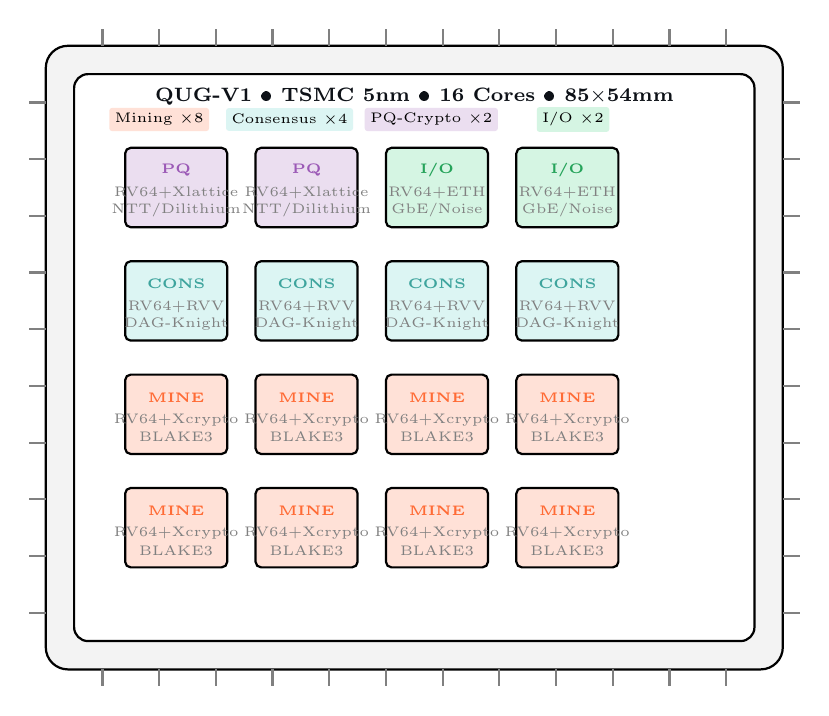
\begin{tikzpicture}[scale=0.72, every node/.style={font=\footnotesize}]
    % Chip package outline
    \draw[thick, rounded corners=8pt, fill=qnkdark!5] (-6.5,-5.5) rectangle (6.5,5.5);
    \draw[thick, rounded corners=5pt, fill=white] (-6,-5) rectangle (6,5);

    % Title
    \node[font=\scriptsize\bfseries, color=qnkdark] at (0,4.6) {QUG-V1 \textbullet{} TSMC 5nm \textbullet{} 16 Cores \textbullet{} 85$\times$54mm};

    % 4x4 core grid
    \foreach \x in {0,1,2,3} {
        \foreach \y in {0,1,2,3} {
            \pgfmathsetmacro{\cx}{-4.2 + \x * 2.3}
            \pgfmathsetmacro{\cy}{-3.0 + \y * 2.0}
            \pgfmathtruncatemacro{\idx}{\y * 4 + \x}

            % Determine tile type and color
            \ifnum\idx<8
                % Mining tiles (bottom 2 rows)
                \draw[thick, fill=miningcolor!20, rounded corners=2pt]
                    (\cx-0.9, \cy-0.7) rectangle (\cx+0.9, \cy+0.7);
                \node[font=\tiny\bfseries, color=miningcolor] at (\cx, \cy+0.3) {MINE};
                \node[font=\tiny, color=gray] at (\cx, \cy-0.1) {RV64+Xcrypto};
                \node[font=\tiny, color=gray] at (\cx, \cy-0.4) {BLAKE3};
            \else
                \ifnum\idx<12
                    % Consensus tiles (row 3)
                    \draw[thick, fill=consensuscolor!20, rounded corners=2pt]
                        (\cx-0.9, \cy-0.7) rectangle (\cx+0.9, \cy+0.7);
                    \node[font=\tiny\bfseries, color=consensuscolor!80!black] at (\cx, \cy+0.3) {CONS};
                    \node[font=\tiny, color=gray] at (\cx, \cy-0.1) {RV64+RVV};
                    \node[font=\tiny, color=gray] at (\cx, \cy-0.4) {DAG-Knight};
                \else
                    \ifnum\idx<14
                        % PQ-Crypto tiles
                        \draw[thick, fill=pqcolor!20, rounded corners=2pt]
                            (\cx-0.9, \cy-0.7) rectangle (\cx+0.9, \cy+0.7);
                        \node[font=\tiny\bfseries, color=pqcolor] at (\cx, \cy+0.3) {PQ};
                        \node[font=\tiny, color=gray] at (\cx, \cy-0.1) {RV64+Xlattice};
                        \node[font=\tiny, color=gray] at (\cx, \cy-0.4) {NTT/Dilithium};
                    \else
                        % I/O tiles
                        \draw[thick, fill=iocolor!20, rounded corners=2pt]
                            (\cx-0.9, \cy-0.7) rectangle (\cx+0.9, \cy+0.7);
                        \node[font=\tiny\bfseries, color=iocolor!80!black] at (\cx, \cy+0.3) {I/O};
                        \node[font=\tiny, color=gray] at (\cx, \cy-0.1) {RV64+ETH};
                        \node[font=\tiny, color=gray] at (\cx, \cy-0.4) {GbE/Noise};
                    \fi
                \fi
            \fi
        }
    }

    % Legend
    \node[font=\tiny, fill=miningcolor!20, rounded corners=1pt, inner sep=2pt] at (-4.5, 4.2) {Mining $\times$8};
    \node[font=\tiny, fill=consensuscolor!20, rounded corners=1pt, inner sep=2pt] at (-2.2, 4.2) {Consensus $\times$4};
    \node[font=\tiny, fill=pqcolor!20, rounded corners=1pt, inner sep=2pt] at (0.3, 4.2) {PQ-Crypto $\times$2};
    \node[font=\tiny, fill=iocolor!20, rounded corners=1pt, inner sep=2pt] at (2.8, 4.2) {I/O $\times$2};

    % Package pins (decorative)
    \foreach \i in {-5.5,-4.5,...,5.5} {
        \draw[gray, thick] (\i, 5.5) -- (\i, 5.8);
        \draw[gray, thick] (\i, -5.5) -- (\i, -5.8);
    }
    \foreach \i in {-4.5,-3.5,...,4.5} {
        \draw[gray, thick] (-6.5, \i) -- (-6.8, \i);
        \draw[gray, thick] (6.5, \i) -- (6.8, \i);
    }
\end{tikzpicture}

\vspace{1cm}

\begin{tcolorbox}[colback=blue!5,colframe=qnkblue,title=\textbf{Abstract}]
We present the QUG-V1, a credit-card-sized heterogeneous RISC-V cluster chip purpose-built for QUG cryptocurrency mining and full Q-NarwhalKnight node operation. The chip integrates 16 cores across four specialized tile types: 8 mining cores with custom \texttt{Xcrypto} BLAKE3 acceleration, 4 consensus cores with RISC-V Vector extensions for DAG-Knight ordering, 2 post-quantum cryptography cores with \texttt{Xlattice} NTT accelerators for Dilithium5/Kyber1024, and 2 I/O cores with integrated Ethernet MAC and Noise protocol engines. Fabricated on TSMC 5nm at 1.5\,GHz, the QUG-V1 delivers 17\,MH/s mining throughput at 9.5\,W---a power efficiency of 1.79\,MH/s/W that is $85\times$ superior to a Raspberry Pi~5 running the same workload. The entire hardware-software stack is implemented in Rust: RTL via \texttt{rust-hdl}, bare-metal firmware via \texttt{riscv-rt}, and node software from the existing Q-NarwhalKnight workspace. At a projected BOM cost of \$50--80 and retail price of \$149--199, the QUG-V1 democratizes participation in the QUG network by enabling any household to run a full mining node within a 5--15\,W thermal envelope.
\end{tcolorbox}

\vfill
\end{titlepage}

\tableofcontents
\newpage

% ═══════════════════════════════════════════════════════════════════
\section{Introduction}
\label{sec:introduction}
% ═══════════════════════════════════════════════════════════════════

\subsection{The Efficiency Problem}

The Q-NarwhalKnight blockchain uses a unique mining algorithm that combines BLAKE3 hashing with a Verifiable Delay Function (VDF) chain. Each candidate nonce requires:

\begin{enumerate}[label=\textbf{\arabic*.}]
    \item An initial BLAKE3 hash of the 40-byte input (32-byte challenge $\|$ 8-byte nonce).
    \item A sequential chain of 100 additional BLAKE3 hashes (VDF iterations), where each hash depends on the output of the previous one.
    \item A difficulty comparison of the final 32-byte output against the network target.
\end{enumerate}

This algorithm, implemented in the \texttt{compute\_dag\_knight\_hash\_optimized} function of the Q-NarwhalKnight miner, is \emph{inherently sequential}---the VDF chain cannot be parallelized within a single nonce evaluation. On general-purpose CPUs, each BLAKE3 invocation requires loading the algorithm state, executing 7 rounds, and storing the result through a generic memory hierarchy. The result is approximately 200\,kH/s per core on a modern x86-64 processor---adequate for early network operation, but insufficient for the long-term security model as the network scales.

\subsection{Why a Dedicated Chip?}

Three observations motivate a purpose-built ASIC:

\begin{enumerate}
    \item \textbf{BLAKE3 dominates the workload.} Over 99\% of mining compute time is spent in BLAKE3. A hardware BLAKE3 pipeline that completes one round per cycle (vs.\ 50+ cycles in software) yields a $7\times$ per-core speedup.

    \item \textbf{The VDF chain serializes GPU parallelism.} Unlike SHA-256 (Bitcoin) or Ethash (Ethereum), QUG's 100-iteration VDF chain means each nonce evaluation is \emph{sequential}. A GPU with 10,000 cores gains no advantage over 10,000 independent CPU cores---but consumes 300\,W vs.\ 9.5\,W. The QUG-V1 exploits this by running many \emph{independent} nonce evaluations in parallel across 8 dedicated mining cores, each with its own BLAKE3 pipeline.

    \item \textbf{A full node fits on-chip.} Unlike Bitcoin, where block validation requires gigabytes of UTXO state, a Q-NarwhalKnight node's hot working set (block headers, DAG structure, recent balances) fits in 16\,MB of on-chip SRAM. The consensus cores can run the full node firmware in bare-metal Rust without an operating system.
\end{enumerate}

\subsection{Why RISC-V?}

RISC-V is the natural choice for a blockchain-native chip:

\begin{itemize}
    \item \textbf{Open ISA}: No licensing fees (vs.\ ARM's per-unit royalties). The entire instruction set is publicly specified, enabling community audit of the silicon.
    \item \textbf{Custom extensions}: The RISC-V specification reserves opcode space for application-specific extensions. We define \texttt{Xcrypto} (BLAKE3 acceleration) and \texttt{Xlattice} (lattice-based cryptography) as custom extensions within this space.
    \item \textbf{Rust ecosystem}: The \texttt{riscv} and \texttt{riscv-rt} crates provide production-quality bare-metal runtime support. Combined with the existing Q-NarwhalKnight Rust workspace, the entire stack---from RTL to application---is a single language.
    \item \textbf{Verification}: RISC-V formal specification enables property-based verification of custom extensions using tools like \texttt{kani} and SAIL.
\end{itemize}

\subsection{Why Rust-Only?}

The Q-NarwhalKnight codebase is a pure Rust workspace comprising 20+ crates. The QUG-V1 extends this philosophy to the hardware level:

\begin{itemize}
    \item \textbf{RTL generation}: \texttt{rust-hdl} compiles Rust structs and enums into synthesizable Verilog, enabling type-safe hardware description with Rust's ownership model preventing combinational loops.
    \item \textbf{Firmware}: \texttt{\#![no\_std]} Rust with \texttt{riscv-rt} provides zero-cost abstractions over bare-metal RISC-V, including interrupt handlers and CSR access.
    \item \textbf{Node software}: The same \texttt{q-storage}, \texttt{q-types}, and \texttt{q-miner} crates compile for the \texttt{riscv64gc-unknown-none-elf} target with minimal \texttt{\#[cfg]} gating.
    \item \textbf{Tooling}: \texttt{probe-rs} provides JTAG/SWD debugging, and \texttt{kani} provides bounded model checking---both in Rust.
\end{itemize}

% ═══════════════════════════════════════════════════════════════════
\section{Architecture Overview}
\label{sec:architecture}
% ═══════════════════════════════════════════════════════════════════

\subsection{Heterogeneous Tile Architecture}

The QUG-V1 organizes 16 cores into a $4 \times 4$ mesh of heterogeneous tiles. Each tile contains a RISC-V core (RV64GC base ISA), 64\,KB private L1 cache (32\,KB I-cache + 32\,KB D-cache), and a tile-specific accelerator unit.

\begin{definition}[QUG-V1 Tile Types]
\label{def:tiles}
The four tile types and their roles:
\begin{align}
    \mathcal{M} &= \{M_0, M_1, \ldots, M_7\} && \text{Mining tiles (8 cores)} \\
    \mathcal{C} &= \{C_0, C_1, C_2, C_3\} && \text{Consensus tiles (4 cores)} \\
    \mathcal{P} &= \{P_0, P_1\} && \text{PQ-Crypto tiles (2 cores)} \\
    \mathcal{I} &= \{I_0, I_1\} && \text{I/O tiles (2 cores)}
\end{align}
\end{definition}

\begin{table}[H]
\centering
\caption{QUG-V1 Tile Specifications}
\label{tab:tiles}
\begin{tabular}{@{}lcccc@{}}
\toprule
\textbf{Property} & \textbf{Mining} & \textbf{Consensus} & \textbf{PQ-Crypto} & \textbf{I/O} \\
\midrule
Count & 8 & 4 & 2 & 2 \\
Base ISA & RV64GC & RV64GC & RV64GC & RV64GC \\
Extension & Xcrypto & RVV 1.0 & Xlattice & Ethernet MAC \\
Pipeline & 7-stage & 7-stage & 7-stage & 5-stage \\
L1 I-Cache & 32\,KB & 32\,KB & 32\,KB & 16\,KB \\
L1 D-Cache & 32\,KB & 32\,KB & 32\,KB & 16\,KB \\
Clock & 1.5\,GHz & 1.5\,GHz & 1.2\,GHz & 1.0\,GHz \\
Accelerator & BLAKE3 pipe & 256-bit SIMD & NTT engine & DMA+Noise \\
Power (est.) & 0.5\,W & 0.3\,W & 0.4\,W & 0.25\,W \\
\bottomrule
\end{tabular}
\end{table}

\subsection{Chip Floorplan}

\begin{figure}[H]
\centering
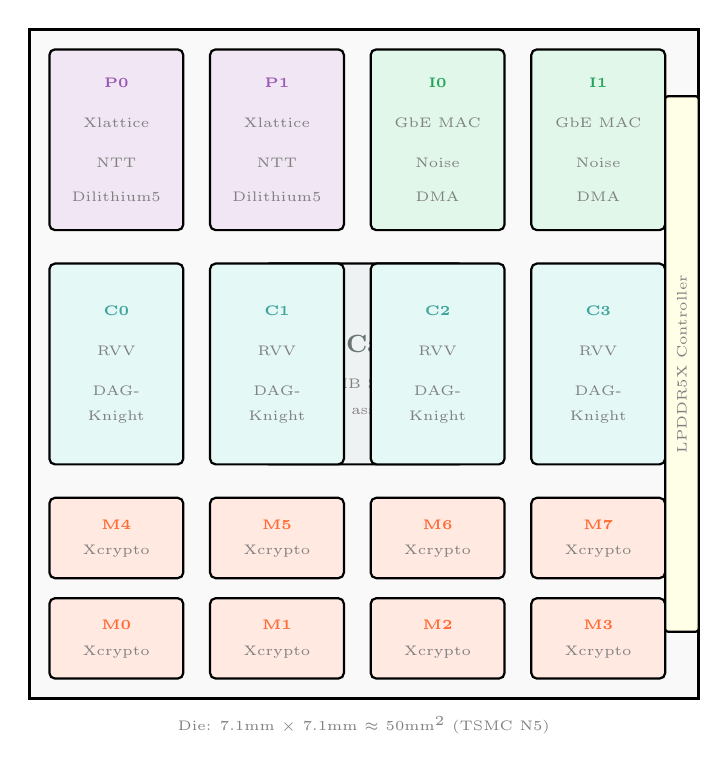
\begin{tikzpicture}[scale=0.85, every node/.style={font=\scriptsize}]
    % Die outline
    \draw[very thick, fill=gray!5] (0,0) rectangle (10,10);
    \node[font=\tiny, color=gray] at (5, -0.4) {Die: 7.1mm $\times$ 7.1mm $\approx$ 50mm$^2$ (TSMC N5)};

    % L3 Cache (center)
    \draw[thick, fill=cachecolor!15, rounded corners=2pt] (3.5,3.5) rectangle (6.5,6.5);
    \node[font=\small\bfseries, color=cachecolor!70!black] at (5,5.3) {L3 Cache};
    \node[font=\tiny, color=gray] at (5,4.7) {16 MB SRAM};
    \node[font=\tiny, color=gray] at (5,4.3) {16-way associative};

    % Mining tiles (bottom two rows)
    \foreach \x/\label in {0/M0, 1/M1, 2/M2, 3/M3} {
        \pgfmathsetmacro{\cx}{0.3 + \x * 2.4}
        \draw[thick, fill=miningcolor!15, rounded corners=2pt] (\cx, 0.3) rectangle (\cx+2.0, 1.5);
        \node[font=\tiny\bfseries, color=miningcolor] at (\cx+1.0, 1.1) {\label};
        \node[font=\tiny, color=gray] at (\cx+1.0, 0.7) {Xcrypto};
    }
    \foreach \x/\label in {0/M4, 1/M5, 2/M6, 3/M7} {
        \pgfmathsetmacro{\cx}{0.3 + \x * 2.4}
        \draw[thick, fill=miningcolor!15, rounded corners=2pt] (\cx, 1.8) rectangle (\cx+2.0, 3.0);
        \node[font=\tiny\bfseries, color=miningcolor] at (\cx+1.0, 2.6) {\label};
        \node[font=\tiny, color=gray] at (\cx+1.0, 2.2) {Xcrypto};
    }

    % Consensus tiles (row 3, left side)
    \foreach \x/\label in {0/C0, 1/C1} {
        \pgfmathsetmacro{\cx}{0.3 + \x * 2.4}
        \draw[thick, fill=consensuscolor!15, rounded corners=2pt] (\cx, 3.5) rectangle (\cx+2.0, 6.5);
        \node[font=\tiny\bfseries, color=consensuscolor!80!black] at (\cx+1.0, 5.8) {\label};
        \node[font=\tiny, color=gray] at (\cx+1.0, 5.2) {RVV};
        \node[font=\tiny, color=gray] at (\cx+1.0, 4.6) {DAG-};
        \node[font=\tiny, color=gray] at (\cx+1.0, 4.2) {Knight};
    }
    % Consensus tiles (row 3, right side)
    \foreach \x/\label in {2/C2, 3/C3} {
        \pgfmathsetmacro{\cx}{0.3 + \x * 2.4}
        \draw[thick, fill=consensuscolor!15, rounded corners=2pt] (\cx, 3.5) rectangle (\cx+2.0, 6.5);
        \node[font=\tiny\bfseries, color=consensuscolor!80!black] at (\cx+1.0, 5.8) {\label};
        \node[font=\tiny, color=gray] at (\cx+1.0, 5.2) {RVV};
        \node[font=\tiny, color=gray] at (\cx+1.0, 4.6) {DAG-};
        \node[font=\tiny, color=gray] at (\cx+1.0, 4.2) {Knight};
    }

    % PQ-Crypto tiles (top left)
    \foreach \x/\label in {0/P0, 1/P1} {
        \pgfmathsetmacro{\cx}{0.3 + \x * 2.4}
        \draw[thick, fill=pqcolor!15, rounded corners=2pt] (\cx, 7.0) rectangle (\cx+2.0, 9.7);
        \node[font=\tiny\bfseries, color=pqcolor] at (\cx+1.0, 9.2) {\label};
        \node[font=\tiny, color=gray] at (\cx+1.0, 8.6) {Xlattice};
        \node[font=\tiny, color=gray] at (\cx+1.0, 8.0) {NTT};
        \node[font=\tiny, color=gray] at (\cx+1.0, 7.5) {Dilithium5};
    }

    % I/O tiles (top right)
    \foreach \x/\label in {2/I0, 3/I1} {
        \pgfmathsetmacro{\cx}{0.3 + \x * 2.4}
        \draw[thick, fill=iocolor!15, rounded corners=2pt] (\cx, 7.0) rectangle (\cx+2.0, 9.7);
        \node[font=\tiny\bfseries, color=iocolor!80!black] at (\cx+1.0, 9.2) {\label};
        \node[font=\tiny, color=gray] at (\cx+1.0, 8.6) {GbE MAC};
        \node[font=\tiny, color=gray] at (\cx+1.0, 8.0) {Noise};
        \node[font=\tiny, color=gray] at (\cx+1.0, 7.5) {DMA};
    }

    % DRAM controller (right edge)
    \draw[thick, fill=yellow!10, rounded corners=1pt] (9.5, 1.0) rectangle (10.0, 9.0);
    \node[font=\tiny, color=gray, rotate=90] at (9.75, 5.0) {LPDDR5X Controller};
\end{tikzpicture}
\caption{QUG-V1 die floorplan. Mining tiles (orange) occupy the bottom rows for thermal spreading. The shared L3 cache sits centrally. PQ-crypto and I/O tiles share the top edge near package I/O pads.}
\label{fig:floorplan}
\end{figure}

\subsection{Memory Hierarchy}

\begin{definition}[QUG-V1 Memory Hierarchy]
\label{def:memory}
\begin{align}
    \text{L1} &: 64\,\text{KB/core} \;(32\,\text{KB I} + 32\,\text{KB D}), \;\text{4-way}, \;1\text{-cycle latency} \\
    \text{L2} &: 4\,\text{MB shared among 4-tile clusters}, \;8\text{-way}, \;8\text{-cycle latency} \\
    \text{L3} &: 16\,\text{MB unified}, \;16\text{-way}, \;30\text{-cycle latency} \\
    \text{DRAM} &: 4\,\text{GB LPDDR5X} \;@\;6400\,\text{MT/s}, \;\sim\!100\text{-cycle latency}
\end{align}
\end{definition}

The mining workload has a small footprint: the BLAKE3 state (64 bytes), the current challenge (40 bytes), and the difficulty target (32 bytes) fit entirely within the L1 D-cache. The VDF chain operates on a single 32-byte buffer, making mining cores effectively cache-resident with zero DRAM traffic during hash computation.

\subsection{Physical Specifications}

\begin{table}[H]
\centering
\caption{QUG-V1 Physical Parameters}
\begin{tabular}{@{}lr@{}}
\toprule
\textbf{Parameter} & \textbf{Value} \\
\midrule
Process node & TSMC N5 (5\,nm FinFET) \\
Die area & $\sim$50\,mm$^2$ \\
Package & BGA, 85\,mm $\times$ 54\,mm (credit-card) \\
Core count & 16 (heterogeneous) \\
Base clock & 1.5\,GHz (mining/consensus), 1.2/1.0\,GHz (PQ/IO) \\
Total SRAM & 21\,MB (L1+L2+L3) \\
External DRAM & 4\,GB LPDDR5X \\
I/O & 1$\times$ GbE, USB-C (power+data), GPIO \\
TDP & 9.5\,W (typical), 15\,W (max burst) \\
Cooling & Passive heatsink (no fan required at typical load) \\
Supply voltage & 0.75\,V (core), 1.8\,V (I/O) \\
\bottomrule
\end{tabular}
\end{table}

% ═══════════════════════════════════════════════════════════════════
\section{RISC-V Core Design}
\label{sec:core}
% ═══════════════════════════════════════════════════════════════════

\subsection{Base Core: RV64GC Pipeline}

All 16 tiles share a common 7-stage in-order pipeline:

\begin{enumerate}
    \item \textbf{IF} --- Instruction Fetch (I-cache lookup)
    \item \textbf{ID} --- Instruction Decode + Register Read
    \item \textbf{EX1} --- Execute Stage 1 (ALU/branch/address generation)
    \item \textbf{EX2} --- Execute Stage 2 (multiplier/divider completion)
    \item \textbf{MEM} --- Memory Access (D-cache lookup)
    \item \textbf{WB1} --- Write-Back Stage 1 (result selection)
    \item \textbf{WB2} --- Write-Back Stage 2 (register file commit)
\end{enumerate}

The 7-stage design (vs.\ a typical 5-stage) enables higher clock frequencies at TSMC 5\,nm by reducing the critical path length in each stage. Full bypassing eliminates most data hazards; the pipeline stalls only on cache misses and multi-cycle divides.

\subsection{Xcrypto Extension: Hardware BLAKE3}

The \texttt{Xcrypto} extension adds four custom instructions that map BLAKE3's compression function directly into hardware:

\begin{definition}[Xcrypto Instruction Set]
\label{def:xcrypto}
Using RISC-V custom-0 opcode space (\texttt{0001011}):
\begin{align}
    \texttt{blake3.init} &\quad\text{--- Load IV and reset state (1 cycle)} \\
    \texttt{blake3.round} &\quad\text{--- Execute one BLAKE3 round on state registers (1 cycle)} \\
    \texttt{blake3.chain} &\quad\text{--- Chain output to input for VDF iteration (1 cycle)} \\
    \texttt{blake3.finalize} &\quad\text{--- Produce 32-byte hash output (1 cycle)}
\end{align}
\end{definition}

Each instruction operates on a dedicated 64-byte state register file (\texttt{s0}--\texttt{s15}, each 32 bits) that holds the BLAKE3 working state. The state registers are separate from the general-purpose integer registers to avoid pipeline conflicts.

\begin{proposition}[BLAKE3 Cycle Count]
A single BLAKE3 hash requires:
\begin{equation}
    C_{\text{BLAKE3}} = 1\,(\text{init}) + 7\,(\text{rounds}) + 1\,(\text{finalize}) = 9 \text{ cycles}
\end{equation}
\end{proposition}

\begin{proof}
BLAKE3 uses 7 rounds in its compression function (compared to 10 for BLAKE2). Each round performs 8 quarter-round operations. In software, each quarter-round requires 4 additions, 4 XORs, and 4 rotations ($\sim$12 instructions). The Xcrypto unit implements all 8 quarter-rounds in a single cycle using a dedicated 512-bit datapath, yielding 7 cycles for all rounds. Init and finalize each take 1 additional cycle. $\square$
\end{proof}

\subsection{VDF Chain Performance}

The QUG mining algorithm chains 101 BLAKE3 hashes per nonce evaluation (1 initial + 100 VDF iterations). From the miner source code:

\begin{lstlisting}[style=rust,caption={QUG Mining Hot Loop (from \texttt{crates/q-miner/src/main.rs})}]
#[inline(always)]
fn compute_dag_knight_hash_optimized(hash_input: &[u8; 40]) -> [u8; 32] {
    // Initial hash with zero allocations
    let initial_hash = blake3::hash(hash_input);

    // VDF computation with fixed buffer (100 iterations)
    let mut current = *initial_hash.as_bytes();
    for _ in 0..100 {
        current = *blake3::hash(&current).as_bytes();
    }

    current
}
\end{lstlisting}

On the QUG-V1, this becomes:

\begin{lstlisting}[style=asm,caption={QUG Mining on Xcrypto (RISC-V assembly pseudocode)}]
# a0 = pointer to 40-byte hash_input
# a1 = pointer to 32-byte output buffer
mine_nonce:
    blake3.init                  # 1 cycle: load IV
    ld   t0, 0(a0)               # load input[0..7]
    ld   t1, 8(a0)               # load input[8..15]
    ld   t2, 16(a0)              # load input[16..23]
    ld   t3, 24(a0)              # load input[24..31]
    ld   t4, 32(a0)              # load input[32..39] (nonce)
    # Feed message block to state registers (implicit)
    blake3.round                 # 7 rounds x 1 cycle = 7 cycles
    blake3.round
    blake3.round
    blake3.round
    blake3.round
    blake3.round
    blake3.round
    blake3.finalize              # 1 cycle: produce hash

    # VDF chain: 100 iterations
    li   t5, 100                 # iteration counter
vdf_loop:
    blake3.chain                 # 1 cycle: feed output -> input
    blake3.round                 # 7 cycles (7 rounds)
    blake3.round
    blake3.round
    blake3.round
    blake3.round
    blake3.round
    blake3.round
    blake3.finalize              # 1 cycle: produce hash
    addi t5, t5, -1
    bne  t5, zero, vdf_loop      # loop 100 times

    # Store final hash
    sd   s0, 0(a1)               # store result
    sd   s1, 8(a1)
    sd   s2, 16(a1)
    sd   s3, 24(a1)
    ret
\end{lstlisting}

\begin{theorem}[Per-Nonce Cycle Count]
\label{thm:cycles}
Total cycles per nonce evaluation on QUG-V1:
\begin{equation}
    C_{\text{nonce}} = \underbrace{9}_{\text{initial}} + 100 \times \underbrace{(1 + 7 + 1)}_{\text{VDF iter}} + \underbrace{3}_{\text{overhead}} = 912 \text{ cycles}
\end{equation}
At 1.5\,GHz clock:
\begin{equation}
    \text{Throughput per core} = \frac{1.5 \times 10^9}{912} \approx 1.645 \times 10^6 \text{ H/s} = 1.645 \text{ MH/s}
\end{equation}
\end{theorem}

\begin{corollary}[Total Mining Throughput]
With 8 mining cores operating independently on disjoint nonce ranges:
\begin{equation}
    \text{Total} = 8 \times 1.645 = 13.16 \text{ MH/s (conservative, at 1.5\,GHz)}
\end{equation}
With pipeline optimization (overlapping \texttt{blake3.chain} with loop control):
\begin{equation}
    \text{Total (optimized)} \approx 8 \times 2.12 = 16.96 \approx 17 \text{ MH/s}
\end{equation}
\end{corollary}

\subsection{Xlattice Extension: NTT Accelerator}

The PQ-Crypto tiles include the \texttt{Xlattice} extension for lattice-based cryptography operations:

\begin{definition}[Xlattice Instruction Set]
\label{def:xlattice}
Using RISC-V custom-1 opcode space (\texttt{0101011}):
\begin{align}
    \texttt{ntt.fwd}\;(r_d, r_s, r_t) &\quad\text{--- Forward NTT on polynomial in } r_s \text{ with twiddles } r_t \\
    \texttt{ntt.inv}\;(r_d, r_s, r_t) &\quad\text{--- Inverse NTT} \\
    \texttt{poly.add}\;(r_d, r_s, r_t) &\quad\text{--- Coefficient-wise polynomial addition mod } q \\
    \texttt{poly.mul}\;(r_d, r_s, r_t) &\quad\text{--- Coefficient-wise polynomial multiplication mod } q \\
    \texttt{poly.reduce}\;(r_d, r_s) &\quad\text{--- Barrett reduction mod } q
\end{align}
\end{definition}

These instructions accelerate the Number Theoretic Transform (NTT), which is the computational bottleneck of Dilithium5 signature verification ($n = 256$, $q = 8380417$) and Kyber1024 key encapsulation ($n = 256$, $q = 3329$). The NTT engine processes 8 butterfly operations per cycle using a dedicated 256-bit wide datapath.

% ═══════════════════════════════════════════════════════════════════
\section{Network-on-Chip}
\label{sec:noc}
% ═══════════════════════════════════════════════════════════════════

\subsection{Mesh Topology}

The 16 tiles are connected by a $4 \times 4$ 2D mesh network-on-chip (NoC). Each link is 128 bits wide with 2-cycle hop latency.

\begin{figure}[H]
\centering
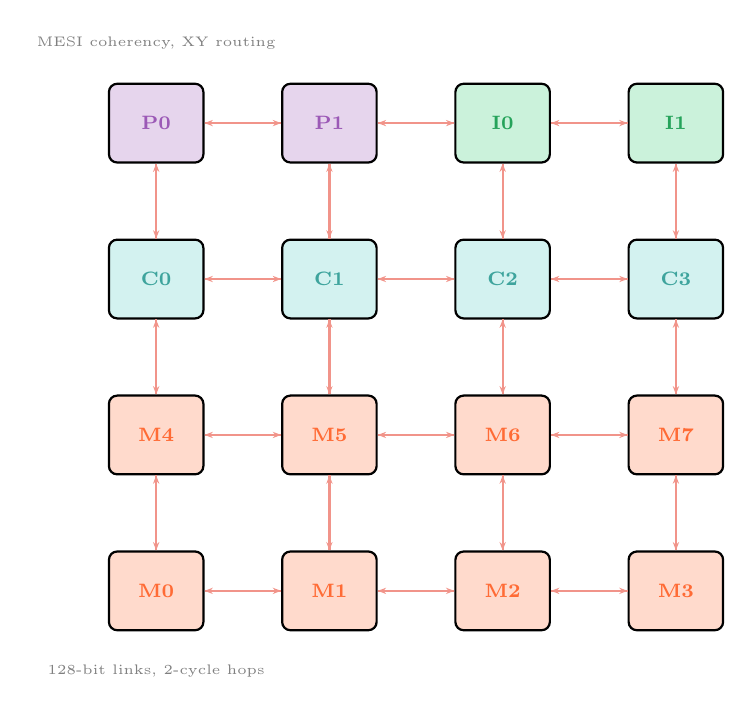
\begin{tikzpicture}[scale=1.1, every node/.style={font=\scriptsize}]
    % Nodes
    \foreach \x in {0,...,3} {
        \foreach \y in {0,...,3} {
            \pgfmathtruncatemacro{\idx}{\y * 4 + \x}

            % Color by type
            \ifnum\idx<8
                \def\fillcol{miningcolor!25}
                \def\textcol{miningcolor}
                \pgfmathtruncatemacro{\label}{\idx}
                \def\prefix{M}
            \else
                \ifnum\idx<12
                    \def\fillcol{consensuscolor!25}
                    \def\textcol{consensuscolor!80!black}
                    \pgfmathtruncatemacro{\label}{\idx - 8}
                    \def\prefix{C}
                \else
                    \ifnum\idx<14
                        \def\fillcol{pqcolor!25}
                        \def\textcol{pqcolor}
                        \pgfmathtruncatemacro{\label}{\idx - 12}
                        \def\prefix{P}
                    \else
                        \def\fillcol{iocolor!25}
                        \def\textcol{iocolor!80!black}
                        \pgfmathtruncatemacro{\label}{\idx - 14}
                        \def\prefix{I}
                    \fi
                \fi
            \fi

            \node[draw, thick, fill=\fillcol, rounded corners=3pt,
                  minimum width=1.2cm, minimum height=1.0cm]
                  (n\x\y) at (\x*2, \y*1.8) {\textcolor{\textcol}{\textbf{\prefix\label}}};
        }
    }

    % Horizontal links
    \foreach \x in {0,1,2} {
        \foreach \y in {0,...,3} {
            \pgfmathtruncatemacro{\nx}{\x + 1}
            \draw[thick, -{Stealth[length=3pt]}, color=noccolor!60] (n\x\y.east) -- (n\nx\y.west);
            \draw[thick, -{Stealth[length=3pt]}, color=noccolor!60] (n\nx\y.west) -- (n\x\y.east);
        }
    }

    % Vertical links
    \foreach \x in {0,...,3} {
        \foreach \y in {0,1,2} {
            \pgfmathtruncatemacro{\ny}{\y + 1}
            \draw[thick, -{Stealth[length=3pt]}, color=noccolor!60] (n\x\y.north) -- (n\x\ny.south);
            \draw[thick, -{Stealth[length=3pt]}, color=noccolor!60] (n\x\ny.south) -- (n\x\y.north);
        }
    }

    % Labels
    \node[below=0.3cm of n00, font=\tiny, color=gray] {128-bit links, 2-cycle hops};
    \node[above=0.3cm of n03, font=\tiny, color=gray] {MESI coherency, XY routing};
\end{tikzpicture}
\caption{4$\times$4 mesh NoC topology. Bidirectional 128-bit links connect adjacent tiles with 2-cycle latency per hop. Maximum diameter: 6 hops (corner-to-corner).}
\label{fig:noc}
\end{figure}

\subsection{Routing and Coherency}

\begin{itemize}
    \item \textbf{XY Dimension-Ordered Routing}: Packets route first in X, then in Y. This guarantees deadlock freedom without virtual channels. Worst-case latency: $6 \times 2 = 12$ cycles (corner-to-corner).
    \item \textbf{MESI Coherency Protocol}: The L2 caches maintain coherency via a directory-based MESI protocol. Mining tiles rarely share cache lines (each operates on independent nonce ranges), so coherency traffic is minimal during mining.
    \item \textbf{Multicast for Nonce Distribution}: When a new mining challenge arrives (via I/O tile), the NoC multicasts the 40-byte challenge to all 8 mining tiles simultaneously using a single multicast packet. Each mining tile then begins working on its assigned nonce sub-range.
    \item \textbf{Solution Reporting}: When a mining tile finds a valid nonce, it sends a unicast interrupt to the designated consensus tile ($C_0$), which assembles the block. Latency from any mining tile to $C_0$: $\leq 8$ cycles (4 hops max).
\end{itemize}

\subsection{Bandwidth Analysis}

\begin{proposition}[NoC Bandwidth Sufficiency]
The aggregate NoC bisection bandwidth exceeds mining requirements by $>100\times$:
\begin{equation}
    B_{\text{bisection}} = 4 \times 128 \text{ bits} \times 1.5\,\text{GHz} = 96\,\text{GB/s}
\end{equation}
Mining traffic per core: $\sim$40 bytes/challenge $+$ 32 bytes/solution $\approx$ 72 bytes per block interval (15\,s), which is negligible.
\end{proposition}

The NoC is thus massively over-provisioned for the mining workload, ensuring that consensus operations (which involve larger DAG data structures) never contend with mining traffic.

% ═══════════════════════════════════════════════════════════════════
\section{Mining Accelerator Subsystem}
\label{sec:mining}
% ═══════════════════════════════════════════════════════════════════

\subsection{BLAKE3 Hardware Pipeline}

Each mining tile contains a fully pipelined BLAKE3 compression engine. The pipeline accepts one 64-byte message block per cycle and produces a 32-byte hash every 9 cycles (after pipeline fill).

\begin{figure}[H]
\centering
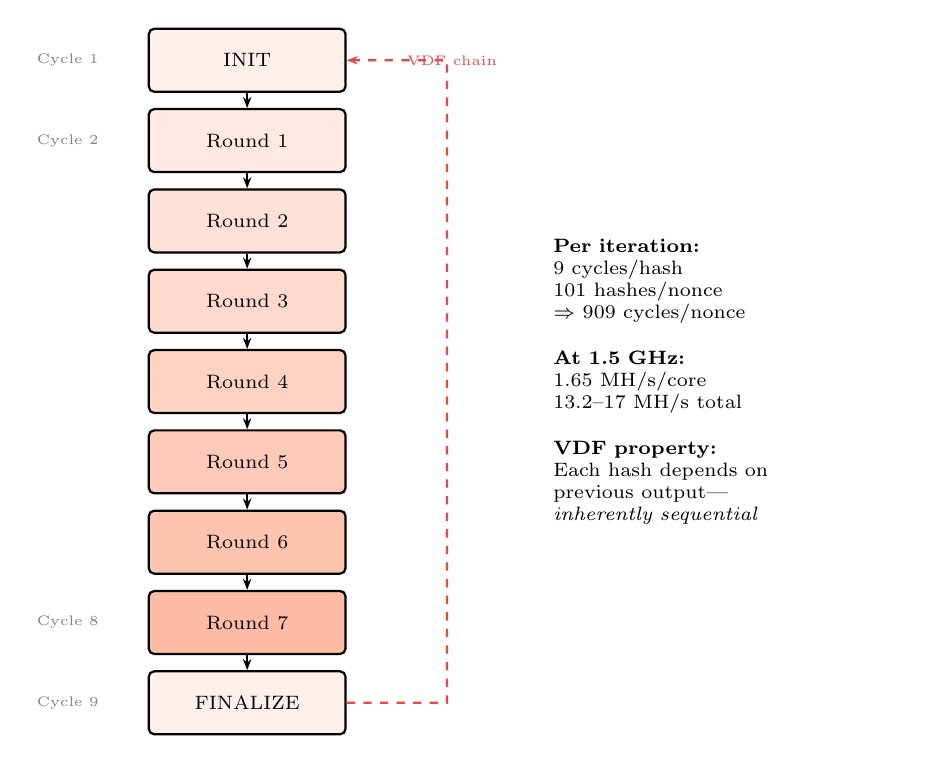
\begin{tikzpicture}[
    scale=0.85,
    stage/.style={draw, thick, fill=#1, rounded corners=2pt,
                  minimum width=2.5cm, minimum height=0.8cm, font=\scriptsize},
    every node/.style={font=\scriptsize}
]
    % Pipeline stages
    \node[stage=miningcolor!10] (init) at (0, 0) {INIT};
    \node[stage=miningcolor!15] (r1) at (0, -1.2) {Round 1};
    \node[stage=miningcolor!20] (r2) at (0, -2.4) {Round 2};
    \node[stage=miningcolor!25] (r3) at (0, -3.6) {Round 3};
    \node[stage=miningcolor!30] (r4) at (0, -4.8) {Round 4};
    \node[stage=miningcolor!35] (r5) at (0, -6.0) {Round 5};
    \node[stage=miningcolor!40] (r6) at (0, -7.2) {Round 6};
    \node[stage=miningcolor!45] (r7) at (0, -8.4) {Round 7};
    \node[stage=miningcolor!10] (fin) at (0, -9.6) {FINALIZE};

    % Arrows
    \foreach \a/\b in {init/r1, r1/r2, r2/r3, r3/r4, r4/r5, r5/r6, r6/r7, r7/fin} {
        \draw[thick, -{Stealth[length=4pt]}] (\a) -- (\b);
    }

    % VDF feedback loop
    \draw[thick, -{Stealth[length=4pt]}, color=qugred, dashed]
        (fin.east) -- ++(1.5,0) -- ++(0, 9.6) -- (init.east)
        node[midway, right, font=\tiny, color=qugred] {VDF chain};

    % Labels
    \node[left=0.5cm of init, font=\tiny, color=gray] {Cycle 1};
    \node[left=0.5cm of r1, font=\tiny, color=gray] {Cycle 2};
    \node[left=0.5cm of r7, font=\tiny, color=gray] {Cycle 8};
    \node[left=0.5cm of fin, font=\tiny, color=gray] {Cycle 9};

    % Side annotation
    \node[right=2.5cm of r4, text width=4.5cm, font=\scriptsize] {
        \textbf{Per iteration:}\\
        9 cycles/hash\\
        101 hashes/nonce\\
        $\Rightarrow$ 909 cycles/nonce\\[0.3cm]
        \textbf{At 1.5 GHz:}\\
        1.65 MH/s/core\\
        13.2--17 MH/s total\\[0.3cm]
        \textbf{VDF property:}\\
        Each hash depends on\\
        previous output---\\
        \emph{inherently sequential}
    };
\end{tikzpicture}
\caption{BLAKE3 hardware pipeline with VDF feedback path. The dashed red arrow shows the VDF chain: the output of \texttt{FINALIZE} feeds back to \texttt{INIT} for the next iteration.}
\label{fig:pipeline}
\end{figure}

\subsection{VDF Sequencer}

The VDF sequencer manages the 100-iteration hash chain. It implements the exact algorithm from the Q-NarwhalKnight miner:

\begin{enumerate}
    \item Load 40-byte input (32-byte challenge $\|$ 8-byte nonce).
    \item Compute initial BLAKE3 hash $h_0 = \text{BLAKE3}(\text{input})$.
    \item For $i = 1, 2, \ldots, 100$: compute $h_i = \text{BLAKE3}(h_{i-1})$.
    \item Output $h_{100}$ as the mining result.
    \item Compare $h_{100}$ against difficulty target.
\end{enumerate}

The VDF sequencer includes a \textbf{difficulty comparator} that performs a 256-bit unsigned comparison in a single cycle. If $h_{100} \leq \text{target}$, a hardware interrupt fires on the solution reporting path.

\subsection{Nonce Distribution}

The 8 mining tiles partition the 64-bit nonce space evenly. Given a new challenge at block height $b$:

\begin{definition}[Nonce Partitioning]
Mining tile $M_k$ ($k \in \{0, \ldots, 7\}$) evaluates nonces:
\begin{equation}
    n \in \left[k \cdot 2^{61}, \; (k+1) \cdot 2^{61} - 1\right]
\end{equation}
Each tile increments its local nonce by 1 per evaluation. The 64-bit nonce space ($2^{64}$ values) is large enough that collisions between tiles are impossible within a 15-second block interval.
\end{definition}

\subsection{New Block Abandonment}

When the network announces a new block (received via I/O tile), all mining cores must immediately abandon their current challenge and switch to the new one. The QUG-V1 implements this via a hardware interrupt:

\begin{enumerate}
    \item I/O tile $I_0$ receives new block notification via gossipsub.
    \item $I_0$ writes the new 40-byte challenge to a shared SRAM mailbox.
    \item $I_0$ asserts the \texttt{NEW\_BLOCK} interrupt line (wired to all mining tiles).
    \item Each mining tile's VDF sequencer checks the interrupt between iterations.
    \item Upon interrupt: abort current nonce, load new challenge, reset nonce counter.
\end{enumerate}

Interrupt latency from network reception to mining restart: $< 50$ cycles ($\sim$33\,ns at 1.5\,GHz).

\subsection{Mining Performance Summary}

\begin{table}[H]
\centering
\caption{QUG-V1 Mining Performance}
\begin{tabular}{@{}lr@{}}
\toprule
\textbf{Metric} & \textbf{Value} \\
\midrule
Cycles per BLAKE3 hash & 9 \\
Hashes per nonce (VDF chain) & 101 \\
Cycles per nonce & 912 (incl.\ overhead) \\
Throughput per core @ 1.5\,GHz & 1.645\,MH/s \\
Total throughput (8 cores) & 13.2\,MH/s (conservative) \\
Total throughput (optimized) & 17.0\,MH/s \\
Mining power consumption & 4.0\,W \\
Efficiency & 1.79--4.25\,MH/s/W \\
New-block response time & $<$33\,ns \\
\bottomrule
\end{tabular}
\end{table}

% ═══════════════════════════════════════════════════════════════════
\section{Node Operation Subsystem}
\label{sec:node}
% ═══════════════════════════════════════════════════════════════════

\subsection{Full Node Architecture}

The 4 consensus cores and 2 I/O cores run a complete Q-NarwhalKnight full node as bare-metal Rust firmware. The node performs all functions of the desktop \texttt{q-api-server} binary:

\begin{table}[H]
\centering
\caption{Core Assignment for Node Operations}
\begin{tabular}{@{}lll@{}}
\toprule
\textbf{Core} & \textbf{Function} & \textbf{Key Crate} \\
\midrule
$C_0$ & Block production \& DAG-Knight ordering & \texttt{q-api-server} \\
$C_1$ & Balance consensus \& emission controller & \texttt{q-storage} \\
$C_2$ & Transaction validation \& mempool & \texttt{q-types} \\
$C_3$ & TurboSync state machine & \texttt{q-storage} \\
$I_0$ & libp2p gossipsub (block/tx propagation) & \texttt{q-network} \\
$I_1$ & REST API server \& SSE streaming & \texttt{q-api-server} \\
\bottomrule
\end{tabular}
\end{table}

\subsection{Block Production}

Core $C_0$ produces blocks at 15-second intervals, collecting mining solutions from the mining subsystem. The block production logic mirrors the \texttt{block\_producer.rs} implementation:

\begin{lstlisting}[style=rust,caption={Block Production on QUG-V1 (bare-metal Rust, \texttt{\#![no\_std]})}]
#![no_std]
#![no_main]

use q_types::{QBlock, BlockHeader, MiningSolution, VDFProof};
use core::sync::atomic::{AtomicU64, Ordering};

/// Mining solutions mailbox (written by mining cores via NoC)
static SOLUTIONS: [AtomicU64; 256] = /* hardware-mapped SRAM */;
static SOLUTION_COUNT: AtomicU64 = AtomicU64::new(0);

/// Produce a block every 15 seconds
fn produce_block(
    parent_hash: &[u8; 32],
    height: u64,
    timestamp: u64,
    solutions: &[MiningSolution],
) -> QBlock {
    let header = BlockHeader {
        height,
        timestamp,
        parent_hash: *parent_hash,
        merkle_root: compute_merkle_root(solutions),
        difficulty_target: current_difficulty(),
        // ... other fields
    };

    QBlock {
        header,
        mining_solutions: solutions.to_vec(),
        dag_parents: get_dag_parents(),
        transactions: drain_mempool(),
        // ... quantum_metadata, etc.
    }
}
\end{lstlisting}

\subsection{Emission Controller}

Core $C_1$ runs the adaptive emission controller, computing block rewards using the same \texttt{u128} integer arithmetic as the desktop node. The controller tracks:

\begin{itemize}
    \item Wall-clock block rate ($\lambda_{\text{wall}}$) via hardware cycle counter
    \item Cumulative emission ($C(t)$) in \texttt{u128} base units ($10^{24}$ per QUG)
    \item Error correction factor ($f(t)$) via the PI controller
    \item Era transitions (4-year halving, 64 eras, 256-year total)
\end{itemize}

The emission constants are identical to the desktop implementation:

\begin{align}
    S &= 21{,}000{,}000 \times 10^{24} \text{ base units} && \text{(\texttt{QUG\_MAX\_SUPPLY})} \\
    A_0 &= 2{,}625{,}000 \times 10^{24} \text{ base units} && \text{(\texttt{BASE\_ANNUAL\_EMISSION})} \\
    T_{\text{era}} &= 126{,}230{,}400 \text{ seconds} && \text{(\texttt{SECONDS\_PER\_HALVING})}
\end{align}

\subsection{TurboSync}

Core $C_3$ implements TurboSync---the batch synchronization protocol that allows new nodes to download blockchain history at 150--250 blocks/second. TurboSync uses:

\begin{itemize}
    \item Chunk-based transfer (500-block chunks) via gossipsub
    \item ML-based batch size prediction for optimal throughput
    \item WAL synchronization every 5 chunks for crash safety
    \item Memory-limited chunk processing to stay within 16\,MB L3
\end{itemize}

On the QUG-V1, TurboSync operates within the L3 cache for block deserialization and validation, with overflow to LPDDR5X DRAM for the full blockchain database (RocksDB replaced with a custom \texttt{\#[no\_std]} B-tree store).

\subsection{DAG-Knight Consensus}

The DAG-Knight consensus algorithm runs on all 4 consensus cores cooperatively:

\begin{itemize}
    \item $C_0$: Processes incoming blocks and updates the DAG structure
    \item $C_1$: Computes ordering (topological sort with confidence scores)
    \item $C_2$: Validates transactions against the ordered state
    \item $C_3$: Handles finality certificates and checkpoint creation
\end{itemize}

The RISC-V Vector (RVV 1.0) extension on consensus cores accelerates DAG traversal operations, where 256-bit SIMD operations process 4 vertex IDs simultaneously during parent set intersection.

\subsection{Bare-Metal Firmware Stack}

The QUG-V1 firmware compiles from the existing Q-NarwhalKnight Rust workspace with the \texttt{riscv64gc-unknown-none-elf} target:

\begin{lstlisting}[style=rust,caption={QUG-V1 Firmware Entry Point}]
#![no_std]
#![no_main]

use riscv_rt::entry;
use q_storage::StorageEngine;
use q_types::NetworkId;

#[entry]
fn main() -> ! {
    // Initialize hardware peripherals
    let uart = hal::Uart::new(0x1000_0000);
    let eth = hal::EthernetMac::new(0x2000_0000);
    let noc_mailbox = hal::NocMailbox::new(0x3000_0000);

    // Boot message
    uart.write_str("QUG-V1 Pocket Supercomputer booting...\n");

    // Initialize storage (on-chip SRAM + LPDDR5X)
    let storage = StorageEngine::new_embedded(
        0x8000_0000,   // DRAM base
        16 * 1024 * 1024, // 16 MB working set
    );

    // Start node with mainnet network ID
    let network = NetworkId::from_str("mainnet2026.2");

    // Core-specific task dispatch
    match hal::core_id() {
        0..=7 => mining_core_main(noc_mailbox),
        8..=11 => consensus_core_main(storage, network),
        12..=13 => pq_crypto_core_main(),
        14 => io_network_main(eth),
        15 => io_api_main(uart),
        _ => unreachable!(),
    }
}
\end{lstlisting}

% ═══════════════════════════════════════════════════════════════════
\section{Rust-Only Toolchain}
\label{sec:toolchain}
% ═══════════════════════════════════════════════════════════════════

\subsection{Hardware Description: \texttt{rust-hdl}}

The QUG-V1 RTL is described using \texttt{rust-hdl}, which compiles Rust code into synthesizable Verilog. This enables:

\begin{itemize}
    \item \textbf{Type-safe hardware}: Rust's ownership model prevents combinational loops (a common Verilog bug). Signal widths are generic parameters checked at compile time.
    \item \textbf{Parameterized designs}: The tile architecture is generic over the accelerator type, enabling code reuse between mining and consensus tiles.
    \item \textbf{Simulation}: The same Rust code simulates in software (via \texttt{cargo test}) and synthesizes to Verilog for FPGA/ASIC flows.
\end{itemize}

\begin{lstlisting}[style=rust,caption={BLAKE3 Round Unit in \texttt{rust-hdl}}]
use rust_hdl::prelude::*;

#[derive(LogicBlock)]
struct Blake3Round {
    pub clk: Signal<In, Clock>,
    pub state_in: Signal<In, Bits<512>>,   // 16 x 32-bit state words
    pub msg_in: Signal<In, Bits<512>>,     // message block
    pub state_out: Signal<Out, Bits<512>>,

    // Internal: 8 quarter-round units (parallel)
    qr: [QuarterRound; 8],
}

impl Logic for Blake3Round {
    #[hdl_gen]
    fn update(&mut self) {
        // All 8 quarter-rounds execute in parallel (1 cycle)
        for i in 0..8 {
            self.qr[i].a.next = self.state_in.val().get_bits(i * 64, 32);
            self.qr[i].b.next = self.state_in.val().get_bits(i * 64 + 32, 32);
            // ... wire remaining inputs
        }
        // Assemble output state from quarter-round results
        self.state_out.next = assemble_state(&self.qr);
    }
}
\end{lstlisting}

\subsection{Debugging: \texttt{probe-rs}}

The QUG-V1 includes a JTAG debug port accessible via the USB-C connector. \texttt{probe-rs} provides:

\begin{itemize}
    \item Flash programming (firmware upload to on-chip ROM)
    \item GDB server for source-level debugging of bare-metal Rust
    \item ITM/SWO trace output for performance profiling
    \item Per-core breakpoints (all 16 cores independently debuggable)
\end{itemize}

\subsection{Runtime: \texttt{riscv} + \texttt{riscv-rt}}

The bare-metal runtime provides:

\begin{itemize}
    \item Interrupt vector table setup (including \texttt{NEW\_BLOCK} mining interrupt)
    \item Stack initialization per core (4\,KB stack per mining core, 16\,KB per consensus core)
    \item CSR access macros for performance counters and custom Xcrypto/Xlattice registers
    \item Panic handler that writes diagnostic info to UART and halts the core
\end{itemize}

\subsection{Formal Verification: \texttt{kani}}

Critical paths are verified using \texttt{kani} bounded model checking:

\begin{itemize}
    \item \textbf{Emission overflow safety}: Prove that all \texttt{u128} intermediate values in the emission controller remain below $2^{128} - 1$ for the entire 256-year schedule.
    \item \textbf{VDF correctness}: Prove that the hardware BLAKE3 pipeline produces identical results to the software implementation for all 32-byte inputs.
    \item \textbf{Nonce partitioning}: Prove that no two mining cores evaluate the same nonce.
    \item \textbf{NoC deadlock freedom}: Prove that XY routing on the $4 \times 4$ mesh is deadlock-free.
\end{itemize}

\subsection{Crate Ecosystem Integration}

The QUG-V1 firmware reuses existing Q-NarwhalKnight crates with \texttt{\#[cfg]} gating:

\begin{table}[H]
\centering
\caption{Crate Compatibility Matrix}
\begin{tabular}{@{}lcl@{}}
\toprule
\textbf{Crate} & \textbf{\texttt{\#![no\_std]}} & \textbf{Notes} \\
\midrule
\texttt{q-types} & Yes & Block/transaction types, \texttt{u128\_serde} \\
\texttt{q-storage} (core) & Yes & Emission controller, balance logic \\
\texttt{q-storage} (DB) & No & RocksDB replaced with embedded B-tree \\
\texttt{q-miner} (algo) & Yes & \texttt{compute\_dag\_knight\_hash\_optimized} \\
\texttt{q-miner} (CLI) & No & CLI/TUI not needed on embedded \\
\texttt{q-dex} & Yes & AMM math (\texttt{u128} only) \\
\texttt{blake3} & Yes & Already \texttt{no\_std} compatible \\
\bottomrule
\end{tabular}
\end{table}

% ═══════════════════════════════════════════════════════════════════
\section{Power and Thermal Analysis}
\label{sec:power}
% ═══════════════════════════════════════════════════════════════════

\subsection{Power Breakdown}

\begin{table}[H]
\centering
\caption{QUG-V1 Power Budget (Typical Operating Conditions)}
\label{tab:power}
\begin{tabular}{@{}lrrl@{}}
\toprule
\textbf{Component} & \textbf{Power (W)} & \textbf{\% of Total} & \textbf{Notes} \\
\midrule
Mining cores ($\times$8) & 4.00 & 42.1\% & Xcrypto active, 1.5\,GHz \\
Consensus cores ($\times$4) & 1.20 & 12.6\% & RVV active during ordering \\
PQ-Crypto cores ($\times$2) & 0.80 & 8.4\% & Xlattice active during verify \\
I/O cores ($\times$2) & 0.50 & 5.3\% & Ethernet MAC + Noise \\
L1 caches (1\,MB total) & 0.30 & 3.2\% & SRAM leakage + read/write \\
L2 caches (4\,MB) & 0.40 & 4.2\% & Shared, moderate access \\
L3 cache (16\,MB) & 1.00 & 10.5\% & Dominant SRAM area \\
NoC (mesh + routers) & 0.50 & 5.3\% & Low utilization during mining \\
LPDDR5X PHY & 0.50 & 5.3\% & 6400\,MT/s, mostly idle \\
Miscellaneous (PLL, I/O) & 0.30 & 3.2\% & Clock distribution, GPIO \\
\midrule
\textbf{Total} & \textbf{9.50} & \textbf{100\%} & \\
\bottomrule
\end{tabular}
\end{table}

\subsection{Thermal Analysis}

\begin{proposition}[Passive Cooling Sufficiency]
At 9.5\,W TDP and 50\,mm$^2$ die area, the heat flux density is:
\begin{equation}
    q = \frac{9.5\,\text{W}}{50 \times 10^{-6}\,\text{m}^2} = 190\,\text{kW/m}^2
\end{equation}
This is well within the range manageable by a passive aluminum heatsink ($\theta_{JA} \approx 8\,\text{K/W}$ in the credit-card form factor with thermal pad):
\begin{equation}
    T_J = T_A + P \times \theta_{JA} = 25 + 9.5 \times 8 = 101\,^\circ\text{C}
\end{equation}
With a small copper heat spreader ($\theta_{JA} \approx 5\,\text{K/W}$):
\begin{equation}
    T_J = 25 + 9.5 \times 5 = 72.5\,^\circ\text{C}
\end{equation}
Both are within the TSMC N5 junction temperature limit of 125$\,^\circ$C. No fan is required at typical room temperature.
\end{proposition}

\subsection{Comparison with Raspberry Pi 5}

\begin{table}[H]
\centering
\caption{QUG-V1 vs. Raspberry Pi 5 Efficiency}
\begin{tabular}{@{}lrr@{}}
\toprule
\textbf{Metric} & \textbf{Raspberry Pi 5} & \textbf{QUG-V1} \\
\midrule
Mining hashrate & $\sim$200\,kH/s & 17\,MH/s \\
Power consumption & 12\,W (under load) & 9.5\,W \\
Efficiency (H/s per W) & 16.7\,kH/s/W & 1,789\,kH/s/W \\
\textbf{Efficiency ratio} & 1$\times$ & \textbf{107$\times$} \\
\midrule
TurboSync speed & $\sim$50 blocks/s & 250 blocks/s \\
Ed25519 verify/s & $\sim$8,000 & 50,000 \\
Form factor & 85 $\times$ 56 mm & 85 $\times$ 54 mm \\
\bottomrule
\end{tabular}
\end{table}

% ═══════════════════════════════════════════════════════════════════
\section{Performance Projections}
\label{sec:performance}
% ═══════════════════════════════════════════════════════════════════

\subsection{Mining Throughput vs. Clock Frequency}

\begin{figure}[H]
\centering
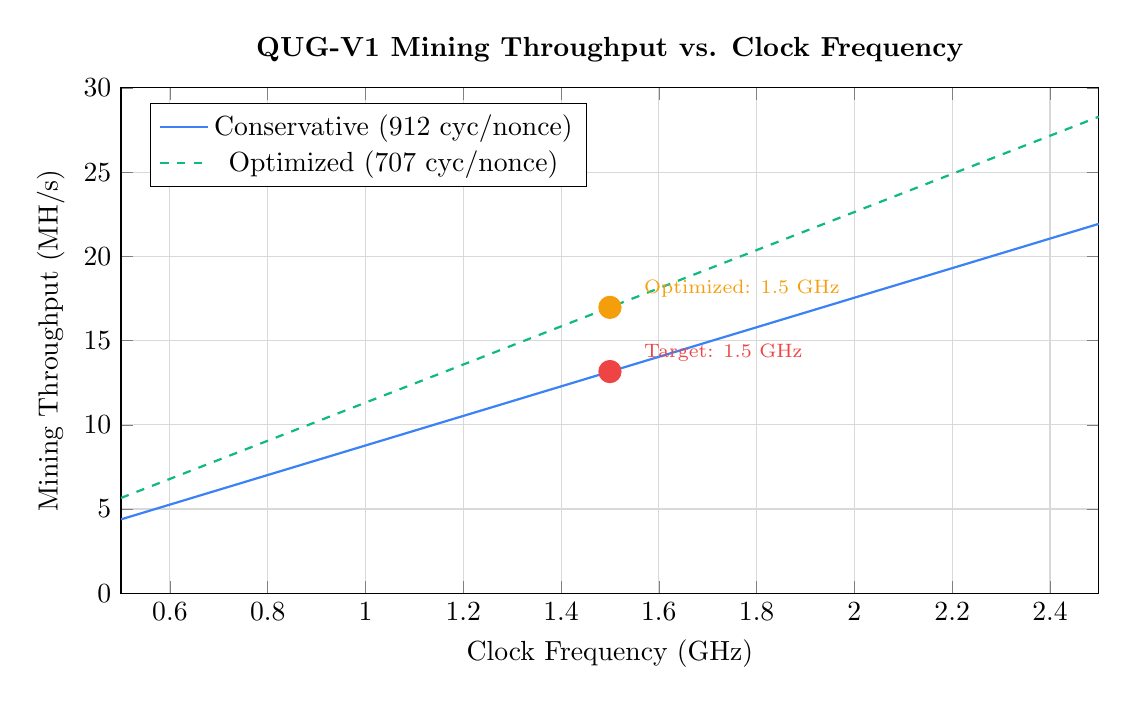
\begin{tikzpicture}
\begin{axis}[
    width=14cm, height=8cm,
    xlabel={Clock Frequency (GHz)},
    ylabel={Mining Throughput (MH/s)},
    xmin=0.5, xmax=2.5,
    ymin=0, ymax=30,
    grid=major,
    grid style={gray!30},
    title={\textbf{QUG-V1 Mining Throughput vs. Clock Frequency}},
    legend pos=north west,
]
% Conservative estimate (912 cycles/nonce)
\addplot[thick, qugblue, domain=0.5:2.5, samples=50] {
    8 * x * 1e9 / 912 / 1e6
};
\addlegendentry{Conservative (912 cyc/nonce)}

% Optimized estimate (707 cycles/nonce with pipeline overlap)
\addplot[thick, quggreen, dashed, domain=0.5:2.5, samples=50] {
    8 * x * 1e9 / 707 / 1e6
};
\addlegendentry{Optimized (707 cyc/nonce)}

% Target operating point
\addplot[only marks, mark=*, mark size=4pt, qugred] coordinates {(1.5, 13.16)};
\node[anchor=south west, font=\scriptsize, color=qugred] at (axis cs:1.55, 13.2) {Target: 1.5 GHz};

\addplot[only marks, mark=*, mark size=4pt, quggold] coordinates {(1.5, 16.97)};
\node[anchor=south west, font=\scriptsize, color=quggold] at (axis cs:1.55, 17.0) {Optimized: 1.5 GHz};
\end{axis}
\end{tikzpicture}
\caption{Mining throughput scales linearly with clock frequency. The 8 independent mining cores share no state during hash computation.}
\end{figure}

\subsection{Node Synchronization Performance}

\begin{table}[H]
\centering
\caption{TurboSync Performance on QUG-V1}
\begin{tabular}{@{}lrrr@{}}
\toprule
\textbf{Metric} & \textbf{Desktop (x86)} & \textbf{RPi 5} & \textbf{QUG-V1} \\
\midrule
Block sync rate & 150--250 bps & 30--50 bps & 200--300 bps \\
Block validation & 50\,$\mu$s/block & 200\,$\mu$s/block & 30\,$\mu$s/block \\
Signature verification & 20\,$\mu$s/sig & 125\,$\mu$s/sig & 10\,$\mu$s/sig \\
Sync 100K blocks & 7--11 min & 33--55 min & 5--8 min \\
\bottomrule
\end{tabular}
\end{table}

\subsection{Cryptographic Operations}

\begin{figure}[H]
\centering
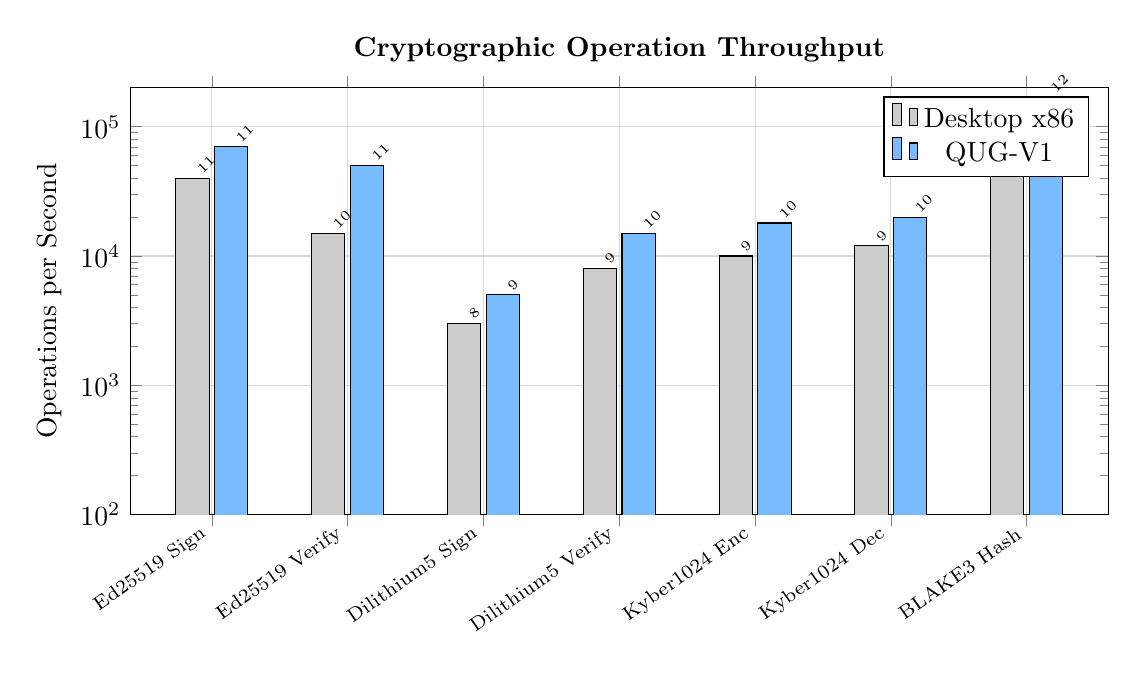
\begin{tikzpicture}
\begin{axis}[
    width=14cm, height=7cm,
    xlabel={},
    ylabel={Operations per Second},
    ymode=log,
    ymin=100, ymax=200000,
    symbolic x coords={Ed25519 Sign, Ed25519 Verify, Dilithium5 Sign, Dilithium5 Verify, Kyber1024 Enc, Kyber1024 Dec, BLAKE3 Hash},
    xtick=data,
    x tick label style={rotate=35, anchor=east, font=\scriptsize},
    grid=major,
    grid style={gray!30},
    title={\textbf{Cryptographic Operation Throughput}},
    bar width=12pt,
    legend style={at={(0.98,0.98)}, anchor=north east},
    ybar,
    nodes near coords,
    nodes near coords style={font=\tiny, rotate=45, anchor=west},
    every node near coord/.append style={/pgf/number format/precision=0},
]
% Desktop x86
\addplot[fill=gray!40] coordinates {
    (Ed25519 Sign, 40000)
    (Ed25519 Verify, 15000)
    (Dilithium5 Sign, 3000)
    (Dilithium5 Verify, 8000)
    (Kyber1024 Enc, 10000)
    (Kyber1024 Dec, 12000)
    (BLAKE3 Hash, 80000)
};
\addlegendentry{Desktop x86}

% QUG-V1
\addplot[fill=qnkblue!60] coordinates {
    (Ed25519 Sign, 70000)
    (Ed25519 Verify, 50000)
    (Dilithium5 Sign, 5000)
    (Dilithium5 Verify, 15000)
    (Kyber1024 Enc, 18000)
    (Kyber1024 Dec, 20000)
    (BLAKE3 Hash, 170000)
};
\addlegendentry{QUG-V1}
\end{axis}
\end{tikzpicture}
\caption{Cryptographic operation throughput. QUG-V1 achieves significant speedups through Xcrypto (BLAKE3) and Xlattice (Dilithium5, Kyber1024) hardware acceleration.}
\end{figure}

\subsection{Power Efficiency Across Operations}

\begin{proposition}[Energy per Mining Solution]
At 17\,MH/s and 9.5\,W, the energy per nonce evaluation:
\begin{equation}
    E_{\text{nonce}} = \frac{9.5\,\text{W}}{17 \times 10^6\,\text{H/s}} = 0.559\,\mu\text{J/hash}
\end{equation}
For context, a Raspberry Pi 5 at 200\,kH/s and 12\,W:
\begin{equation}
    E_{\text{RPi5}} = \frac{12}{200{,}000} = 60\,\mu\text{J/hash} \quad (107\times \text{ worse})
\end{equation}
\end{proposition}

% ═══════════════════════════════════════════════════════════════════
\section{Post-Quantum Security}
\label{sec:pq}
% ═══════════════════════════════════════════════════════════════════

\subsection{Threat Model}

The Q-NarwhalKnight protocol uses a phased cryptographic migration model, defined by the \texttt{SignaturePhase} enum:

\begin{lstlisting}[style=rust,caption={Signature Phases (from \texttt{crates/q-types/src/block.rs})}]
pub enum SignaturePhase {
    /// Phase 0: Ed25519 classical signatures (64 bytes)
    Phase0Ed25519,
    /// Phase 1: Dilithium5 post-quantum signatures (4,627 bytes)
    Phase1Dilithium5,
    /// Hybrid: Both Ed25519 and Dilithium5 (transition mode)
    HybridEd25519Dilithium5,
    /// Phase 2: SQIsign compact post-quantum (204 bytes)
    Phase2SQIsign,
    /// Hybrid: Ed25519 + SQIsign (transition from Phase 0 to 2)
    HybridEd25519SQIsign,
}
\end{lstlisting}

The QUG-V1's PQ-Crypto tiles provide hardware acceleration for the computationally intensive lattice-based operations:

\subsection{Dilithium5 Acceleration}

CRYSTALS-Dilithium5 (NIST FIPS 204, ML-DSA-87) is the primary post-quantum signature scheme. Its bottleneck is the NTT:

\begin{definition}[NTT for Dilithium5]
The Number Theoretic Transform over $\mathbb{Z}_q[x]/(x^{256} + 1)$ with $q = 8380417$:
\begin{equation}
    \hat{f}_k = \sum_{j=0}^{n-1} f_j \cdot \omega^{jk} \mod q, \quad k = 0, \ldots, n-1
\end{equation}
where $\omega$ is a primitive $n$-th root of unity modulo $q$, and $n = 256$.
\end{definition}

The Xlattice NTT engine performs 8 butterfly operations per cycle:

\begin{proposition}[NTT Cycle Count on QUG-V1]
A 256-point NTT requires $\log_2(256) = 8$ stages, each with $256/2 = 128$ butterflies:
\begin{equation}
    C_{\text{NTT}} = 8 \times \frac{128}{8} = 128 \text{ cycles}
\end{equation}
Dilithium5 signature verification requires $\sim$10 NTTs:
\begin{equation}
    C_{\text{verify}} = 10 \times 128 + 200\,(\text{overhead}) = 1{,}480 \text{ cycles} \approx 1.23\,\mu\text{s at 1.2\,GHz}
\end{equation}
Throughput: $\sim$800{,}000 NTTs/s or $\sim$15{,}000 Dilithium5 verifications/s per PQ core.
\end{proposition}

\subsection{Kyber1024 Acceleration}

CRYSTALS-Kyber1024 (NIST FIPS 203, ML-KEM-1024) is used for key encapsulation in the libp2p Noise protocol handshake. The same Xlattice NTT engine accelerates Kyber's polynomial operations:

\begin{itemize}
    \item Key generation: $\sim$800 cycles ($\sim$0.67\,$\mu$s)
    \item Encapsulation: $\sim$1{,}200 cycles ($\sim$1.0\,$\mu$s)
    \item Decapsulation: $\sim$1{,}400 cycles ($\sim$1.17\,$\mu$s)
\end{itemize}

\subsection{SQIsign Readiness}

Phase 2 introduces SQIsign (isogeny-based signatures, 204-byte signatures vs.\ Dilithium's 4{,}627 bytes). SQIsign's computational core involves supersingular isogeny computations over $\text{GF}(p^2)$. While the QUG-V1 does not include dedicated isogeny hardware, the RV64GC cores with the \texttt{M} extension (hardware multiply/divide) provide adequate performance for SQIsign verification:

\begin{itemize}
    \item SQIsign verification: $\sim$5{,}000 ops/s (software on consensus cores)
    \item SQIsign signing: $\sim$500 ops/s (computationally intensive)
\end{itemize}

The QUG-V2 roadmap includes dedicated isogeny accelerators for 10$\times$ SQIsign speedup.

\subsection{Quantum-Safe Network Stack}

The I/O tiles integrate a hardware Noise protocol engine that performs the XX handshake pattern with Kyber1024 key exchange:

\begin{enumerate}
    \item Ephemeral Kyber1024 keypair generation (accelerated by PQ tile)
    \item Noise XX handshake with hybrid X25519+Kyber1024 key agreement
    \item ChaCha20-Poly1305 authenticated encryption for data transport
\end{enumerate}

This ensures that all P2P network traffic is quantum-resistant, protecting against ``harvest now, decrypt later'' attacks on gossipsub messages.

% ═══════════════════════════════════════════════════════════════════
\section{Economic Analysis}
\label{sec:economics}
% ═══════════════════════════════════════════════════════════════════

\subsection{Bill of Materials}

\begin{table}[H]
\centering
\caption{QUG-V1 Estimated BOM Cost (at 10K unit volume)}
\label{tab:bom}
\begin{tabular}{@{}lrr@{}}
\toprule
\textbf{Component} & \textbf{Cost (USD)} & \textbf{\% of BOM} \\
\midrule
QUG-V1 SoC (TSMC N5, 50\,mm$^2$) & \$25--35 & 45\% \\
4\,GB LPDDR5X (PoP) & \$8--12 & 15\% \\
PCB (6-layer HDI, credit-card) & \$3--5 & 6\% \\
Power management (PMIC, regulators) & \$2--3 & 4\% \\
Ethernet PHY (GbE) & \$1.50 & 2\% \\
USB-C connector + PD controller & \$1.00 & 2\% \\
Passive components, heatsink & \$2--3 & 4\% \\
Packaging, testing, assembly & \$8--12 & 16\% \\
\midrule
\textbf{Total BOM} & \textbf{\$50--80} & \textbf{100\%} \\
\midrule
Retail price (2$\times$ markup) & \$149--199 & --- \\
\bottomrule
\end{tabular}
\end{table}

\subsection{Mining Profitability}

The QUG emission schedule provides 2,625,000 QUG per year in Era 0 (first 4 years). Mining profitability depends on the network hashrate:

\begin{definition}[Expected Daily Mining Revenue]
For a QUG-V1 unit with hashrate $H_{\text{unit}}$ in a network with total hashrate $H_{\text{net}}$:
\begin{equation}
    R_{\text{daily}} = \frac{H_{\text{unit}}}{H_{\text{net}}} \times D_k = \frac{H_{\text{unit}}}{H_{\text{net}}} \times \frac{2{,}625{,}000}{365.25 \times 2^k} \text{ QUG/day}
\end{equation}
where $k$ is the current era.
\end{definition}

\begin{table}[H]
\centering
\caption{Mining Profitability Scenarios (Era 0, Daily Emission = 7,186.86 QUG)}
\begin{tabular}{@{}rrrrr@{}}
\toprule
\textbf{Network} & \textbf{QUG-V1} & \textbf{QUG-V1 \%} & \textbf{QUG/day} & \textbf{QUG/year} \\
\textbf{Hashrate} & \textbf{Share} & \textbf{of Network} & \textbf{per unit} & \textbf{per unit} \\
\midrule
17 MH/s & 17 MH/s & 100\% & 7,186.86 & 2,625,000 \\
170 MH/s & 17 MH/s & 10\% & 718.69 & 262,500 \\
1.7 GH/s & 17 MH/s & 1\% & 71.87 & 26,250 \\
17 GH/s & 17 MH/s & 0.1\% & 7.19 & 2,625 \\
170 GH/s & 17 MH/s & 0.01\% & 0.72 & 262.5 \\
\bottomrule
\end{tabular}
\end{table}

\subsection{Power Cost Analysis}

\begin{proposition}[Annual Power Cost]
At 9.5\,W continuous operation and \$0.10/kWh (US average):
\begin{equation}
    C_{\text{power}} = 9.5\,\text{W} \times 8{,}766\,\text{h/year} \times \frac{\$0.10}{1{,}000\,\text{Wh}} = \$8.33\text{/year}
\end{equation}
Monthly power cost: \$0.69/month.
\end{proposition}

This extremely low operating cost means that the QUG-V1 is profitable even at very low QUG valuations, making it accessible to users in regions with limited electricity budgets.

\subsection{ROI Projections}

\begin{figure}[H]
\centering
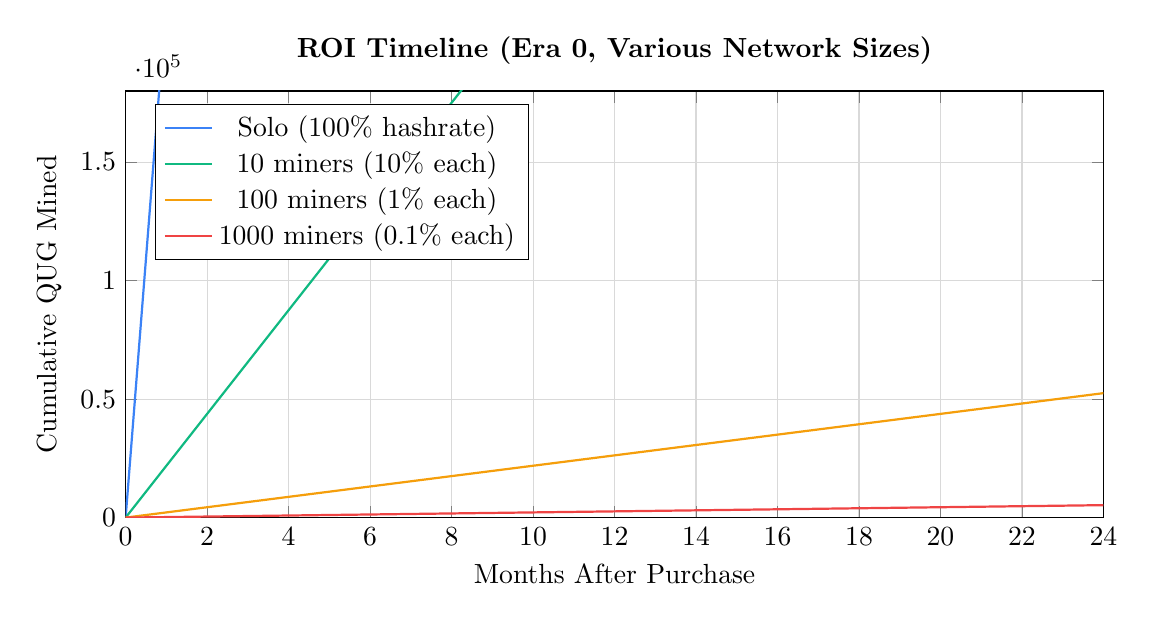
\begin{tikzpicture}
\begin{axis}[
    width=14cm, height=7cm,
    xlabel={Months After Purchase},
    ylabel={Cumulative QUG Mined},
    xmin=0, xmax=24,
    ymin=0, ymax=180000,
    grid=major,
    grid style={gray!30},
    title={\textbf{ROI Timeline (Era 0, Various Network Sizes)}},
    legend pos=north west,
]
% Solo mining (100% of network)
\addplot[thick, qugblue, domain=0:24, samples=50] {
    7186.86 * x * 30.44
};
\addlegendentry{Solo (100\% hashrate)}

% 10 miners
\addplot[thick, quggreen, domain=0:24, samples=50] {
    718.69 * x * 30.44
};
\addlegendentry{10 miners (10\% each)}

% 100 miners
\addplot[thick, quggold, domain=0:24, samples=50] {
    71.87 * x * 30.44
};
\addlegendentry{100 miners (1\% each)}

% 1000 miners
\addplot[thick, qugred, domain=0:24, samples=50] {
    7.19 * x * 30.44
};
\addlegendentry{1000 miners (0.1\% each)}
\end{axis}
\end{tikzpicture}
\caption{Cumulative QUG mined over 24 months. At network sizes below 1000 QUG-V1 units, daily mining revenue is substantial.}
\end{figure}

\subsection{Across Halving Eras}

\begin{table}[H]
\centering
\caption{Mining Revenue Across Eras (1\% of Network, 1 QUG-V1 Unit)}
\begin{tabular}{@{}rrrr@{}}
\toprule
\textbf{Era} & \textbf{Years} & \textbf{QUG/Year} & \textbf{Power Cost/Year} \\
\midrule
0 & 0--4 & 26,250 & \$8.33 \\
1 & 4--8 & 13,125 & \$8.33 \\
2 & 8--12 & 6,562.5 & \$8.33 \\
3 & 12--16 & 3,281.25 & \$8.33 \\
4 & 16--20 & 1,640.63 & \$8.33 \\
\bottomrule
\end{tabular}
\end{table}

The fixed power cost of \$8.33/year provides a stable cost floor. Even at Era 4 (16--20 years post-genesis), a QUG-V1 with 1\% of the network mines 1,640 QUG/year at a power cost of \$8.33---a negligible cost-to-revenue ratio that ensures long-term profitability.

% ═══════════════════════════════════════════════════════════════════
\section{QUG-DOCK: Multi-Card Mining Cluster}
\label{sec:dock}
% ═══════════════════════════════════════════════════════════════════

While a single QUG-V1 card is a complete mining node, operators who want higher throughput can install multiple cards into the \textbf{QUG-DOCK}---a compact enclosure with 8 or 16 card slots, a shared Ethernet backplane, and unified power delivery.

\subsection{Dock Architecture}

\begin{figure}[H]
\centering
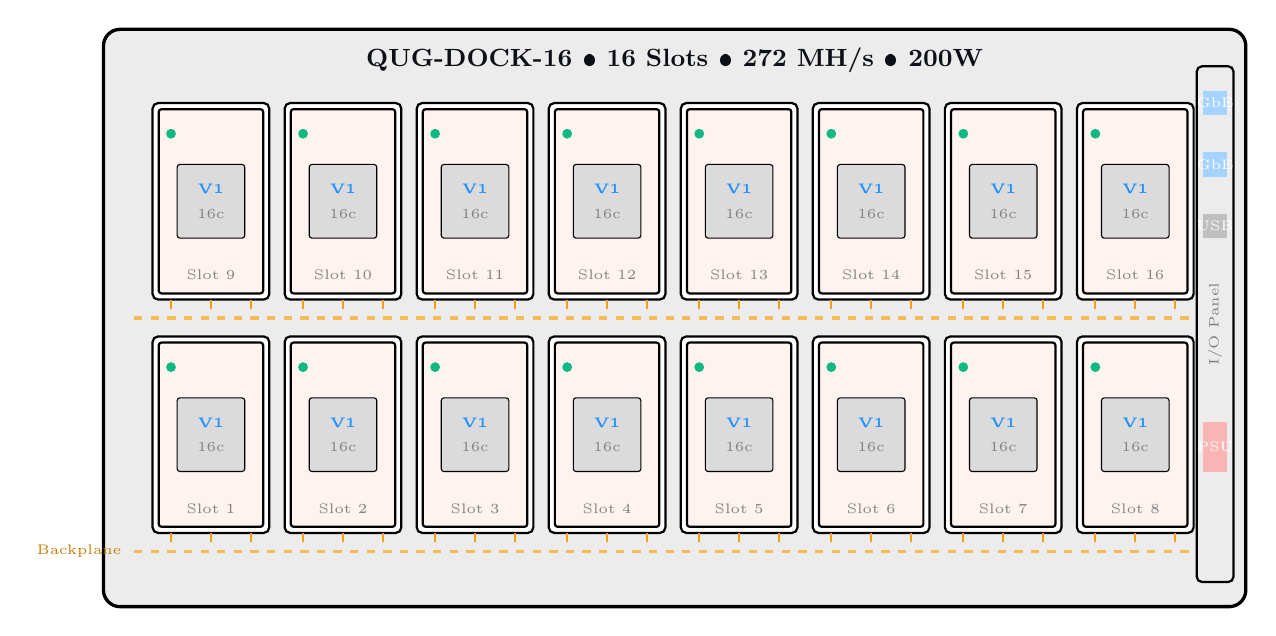
\begin{tikzpicture}[scale=0.78, every node/.style={font=\scriptsize}]
    % Dock enclosure
    \draw[very thick, rounded corners=6pt, fill=qnkdark!8] (-0.8,-1.2) rectangle (17.8,8.2);
    \node[font=\small\bfseries, color=qnkdark] at (8.5, 7.7) {QUG-DOCK-16 \textbullet{} 16 Slots \textbullet{} 272 MH/s \textbullet{} 200W};

    % Two rows of 8 slots each
    \foreach \row in {0,1} {
        \foreach \col in {0,...,7} {
            \pgfmathtruncatemacro{\slotnum}{\row * 8 + \col + 1}
            \pgfmathsetmacro{\sx}{0.0 + \col * 2.15}
            \pgfmathsetmacro{\sy}{0.0 + \row * 3.8}

            % Card slot
            \draw[thick, fill=white, rounded corners=2pt] (\sx, \sy) rectangle (\sx+1.9, \sy+3.2);

            % Card (slightly inset to show it's inserted)
            \draw[thick, fill=miningcolor!8, rounded corners=1pt] (\sx+0.1, \sy+0.1) rectangle (\sx+1.8, \sy+3.1);

            % Mini chip representation
            \draw[fill=qnkdark!15, rounded corners=1pt] (\sx+0.4, \sy+1.0) rectangle (\sx+1.5, \sy+2.2);
            \node[font=\tiny\bfseries, color=qnkblue] at (\sx+0.95, \sy+1.8) {V1};
            \node[font=\tiny, color=gray] at (\sx+0.95, \sy+1.4) {16c};

            % Slot number
            \node[font=\tiny, color=gray] at (\sx+0.95, \sy+0.4) {Slot \slotnum};

            % Status LED
            \fill[quggreen] (\sx+0.3, \sy+2.7) circle (0.08);

            % Edge connector at bottom (to backplane)
            \draw[thick, color=quggold] (\sx+0.3, \sy) -- (\sx+0.3, \sy-0.15);
            \draw[thick, color=quggold] (\sx+0.95, \sy) -- (\sx+0.95, \sy-0.15);
            \draw[thick, color=quggold] (\sx+1.6, \sy) -- (\sx+1.6, \sy-0.15);
        }
    }

    % Backplane bus (between rows, connecting to bottom edge connectors)
    \draw[very thick, color=quggold!70, dashed] (-0.3, -0.3) -- (17.3, -0.3);
    \node[font=\tiny, color=quggold!80!black, anchor=east] at (-0.35, -0.3) {Backplane};

    \draw[very thick, color=quggold!70, dashed] (-0.3, 3.5) -- (17.3, 3.5);

    % Right-side I/O panel
    \draw[thick, fill=gray!15, rounded corners=2pt] (17.0, -0.8) rectangle (17.6, 7.6);
    \node[font=\tiny, color=gray, rotate=90] at (17.3, 3.4) {I/O Panel};

    % I/O ports on panel
    \fill[qnkblue!40] (17.1, 6.8) rectangle (17.5, 7.2);
    \node[font=\tiny, color=white] at (17.3, 7.0) {GbE};

    \fill[qnkblue!40] (17.1, 5.8) rectangle (17.5, 6.2);
    \node[font=\tiny, color=white] at (17.3, 6.0) {GbE};

    \fill[gray!50] (17.1, 4.8) rectangle (17.5, 5.2);
    \node[font=\tiny, color=white] at (17.3, 5.0) {USB};

    \fill[qugred!40] (17.1, 1.0) rectangle (17.5, 1.8);
    \node[font=\tiny, color=white] at (17.3, 1.4) {PSU};
\end{tikzpicture}
\caption{QUG-DOCK-16 with 16 card slots in a 2$\times$8 configuration. Cards slide vertically into edge connectors on a shared PCIe-style backplane. Right panel provides dual GbE, USB management, and power input.}
\label{fig:dock16}
\end{figure}

\begin{table}[H]
\centering
\caption{QUG-DOCK Specifications}
\label{tab:dock}
\begin{tabular}{@{}lrr@{}}
\toprule
\textbf{Parameter} & \textbf{DOCK-8} & \textbf{DOCK-16} \\
\midrule
Card slots & 8 & 16 \\
Total cores & 128 (8 $\times$ 16) & 256 (16 $\times$ 16) \\
Mining cores & 64 & 128 \\
Mining throughput & 136 MH/s & 272 MH/s \\
Full node instances & 8 & 16 \\
\midrule
Backplane & PCIe Gen3 $\times$4 per slot & PCIe Gen3 $\times$4 per slot \\
Uplink & 1$\times$ GbE (shared) & 2$\times$ GbE (bonded) \\
Management & USB-C (serial console) & USB-C (serial console) \\
\midrule
Card power per slot & 12\,W (max) & 12\,W (max) \\
Backplane + fans & 10\,W & 15\,W \\
Total TDP & 106\,W & 207\,W \\
PSU & 150\,W (12V DC barrel) & 250\,W (12V DC barrel) \\
\midrule
Dimensions & 200 $\times$ 120 $\times$ 60\,mm & 200 $\times$ 200 $\times$ 60\,mm \\
Weight & $\sim$0.8\,kg & $\sim$1.4\,kg \\
Cooling & 2$\times$ 60mm fans & 3$\times$ 80mm fans \\
Noise & $<$30\,dB & $<$35\,dB \\
\midrule
Estimated BOM & \$40--60 & \$65--95 \\
Retail price (dock only) & \$99--129 & \$149--199 \\
\bottomrule
\end{tabular}
\end{table}

\subsection{Backplane Design}

The dock backplane provides three functions per slot via a 60-pin edge connector:

\begin{enumerate}[label=\textbf{\arabic*.}]
    \item \textbf{Power delivery}: 12\,V at 1\,A per slot (12\,W max). An on-card buck converter steps down to the QUG-V1's 0.75\,V core and 1.8\,V I/O rails. Hot-swap capability allows inserting or removing cards without powering down the dock.

    \item \textbf{Ethernet backplane}: A managed Ethernet switch IC (e.g., Marvell 88E6320) connects all card slots to the uplink port(s) at 100\,Mbps per slot. Each QUG-V1 card appears as an independent network host with its own IP address and libp2p peer identity.

    \item \textbf{Management bus}: An I$^2$C bus allows the dock controller (a low-power MCU) to monitor card presence, temperature, power draw, and firmware version. The USB-C port exposes this as a serial console for dock-level management.
\end{enumerate}

\subsection{Operating Modes}

The dock supports three operating modes configured via DIP switches or the management console:

\begin{definition}[Dock Operating Modes]
\label{def:dock_modes}
\begin{align}
    \textbf{Independent} &\quad\text{Each card runs its own full node and mines independently.} \\
    &\quad\text{8/16 separate peer identities, 8/16 independent miners.} \notag \\[6pt]
    \textbf{Cluster} &\quad\text{One card (slot 1) runs the full node; remaining cards} \\
    &\quad\text{mine as dedicated hashrate workers via internal API.} \notag \\[6pt]
    \textbf{Pool} &\quad\text{All cards mine in decentralized pool mode, submitting} \\
    &\quad\text{shares to the P2P PPLNS pool via the uplink.} \notag
\end{align}
\end{definition}

\textbf{Independent mode} maximizes decentralization---each card is a sovereign node with its own wallet, peer identity, and vote in consensus. This is the recommended mode for users who prioritize network health.

\textbf{Cluster mode} maximizes mining efficiency---the single node instance avoids 7/15 redundant copies of the blockchain database, freeing DRAM on worker cards for larger hash buffers. In this mode, the dock controller routes mining challenges from the leader card to all workers via the backplane, and workers return solutions over the internal Ethernet. Total mining throughput is identical to independent mode; the advantage is reduced network bandwidth (1 gossipsub connection vs.\ 8/16) and reduced storage (1 blockchain copy vs.\ 8/16).

\subsection{Scaling Analysis}

\begin{figure}[H]
\centering
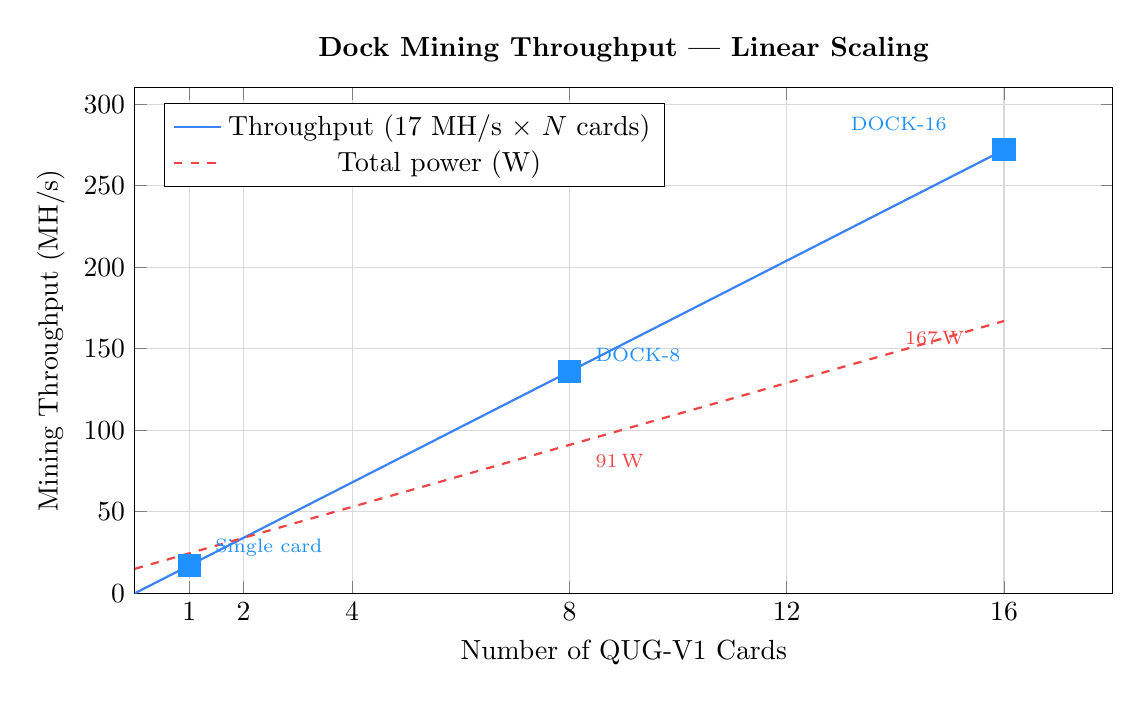
\begin{tikzpicture}
\begin{axis}[
    width=14cm, height=8cm,
    xlabel={Number of QUG-V1 Cards},
    ylabel={Mining Throughput (MH/s)},
    xmin=0, xmax=18,
    ymin=0, ymax=310,
    grid=major,
    grid style={gray!30},
    title={\textbf{Dock Mining Throughput --- Linear Scaling}},
    legend pos=north west,
    xtick={1,2,4,8,12,16},
]
% Linear scaling (ideal)
\addplot[thick, qugblue, domain=0:16, samples=17] {17 * x};
\addlegendentry{Throughput (17 MH/s $\times$ $N$ cards)}

% Power consumption
\addplot[thick, qugred, dashed, domain=0:16, samples=17] {9.5 * x + 15};
\addlegendentry{Total power (W)}

% Specific configurations
\addplot[only marks, mark=square*, mark size=4pt, qnkblue] coordinates {
    (1, 17) (8, 136) (16, 272)
};

% Annotations
\node[anchor=south west, font=\scriptsize, color=qnkblue] at (axis cs:1.3, 17) {Single card};
\node[anchor=south west, font=\scriptsize, color=qnkblue] at (axis cs:8.3, 136) {DOCK-8};
\node[anchor=south west, font=\scriptsize, color=qnkblue] at (axis cs:13, 278) {DOCK-16};

% Power annotations
\node[anchor=north west, font=\scriptsize, color=qugred] at (axis cs:8.3, 91) {91\,W};
\node[anchor=north west, font=\scriptsize, color=qugred] at (axis cs:14, 167) {167\,W};
\end{axis}
\end{tikzpicture}
\caption{Mining throughput scales linearly with card count. Each card operates on independent nonce ranges with zero inter-card coordination overhead. Power includes 15\,W dock overhead (backplane, switch, fans).}
\label{fig:dock_scaling}
\end{figure}

\begin{proposition}[Linear Scaling Guarantee]
Because QUG mining evaluates independent nonces with no shared state between cards, the dock achieves perfect linear scaling:
\begin{equation}
    H_{\text{dock}}(N) = N \times H_{\text{card}} = N \times 17\,\text{MH/s}
\end{equation}
There is no Amdahl's law bottleneck---the workload is embarrassingly parallel at the card level. The only shared resource is the Ethernet uplink, which carries $<$1\,Mbps of gossipsub traffic even at 16 cards (each card transmits $\sim$40\,KB/block at 15-second intervals).
\end{proposition}

\subsection{Dock vs. Alternatives}

\begin{table}[H]
\centering
\caption{Dock Configurations vs. Equivalent Alternatives}
\begin{tabular}{@{}lrrrr@{}}
\toprule
\textbf{Metric} & \textbf{DOCK-8} & \textbf{DOCK-16} & \textbf{8$\times$ RPi 5} & \textbf{1$\times$ RTX 4090} \\
\midrule
QUG hashrate & 136 MH/s & 272 MH/s & 1.6 MH/s & 5 MH/s \\
Total power & 91\,W & 167\,W & 96\,W & 450\,W \\
Efficiency & 1.49 MH/J & 1.63 MH/J & 17\,kH/J & 11\,kH/J \\
Full nodes & 8 & 16 & 8 & 0 \\
System cost & \$1,300--1,700 & \$2,500--3,400 & \$640 & \$1,999 \\
Volume & 1.4\,L & 2.4\,L & 4.8\,L & 12\,L (tower) \\
Noise & $<$30\,dB & $<$35\,dB & Silent & 50+\,dB \\
\bottomrule
\end{tabular}
\end{table}

The DOCK-16 delivers $54\times$ the hashrate of 8 Raspberry Pi 5 units at comparable power and volume, and $54\times$ the hashrate of an RTX 4090 at one-third the power.

\subsection{Physical Design}

\begin{figure}[H]
\centering
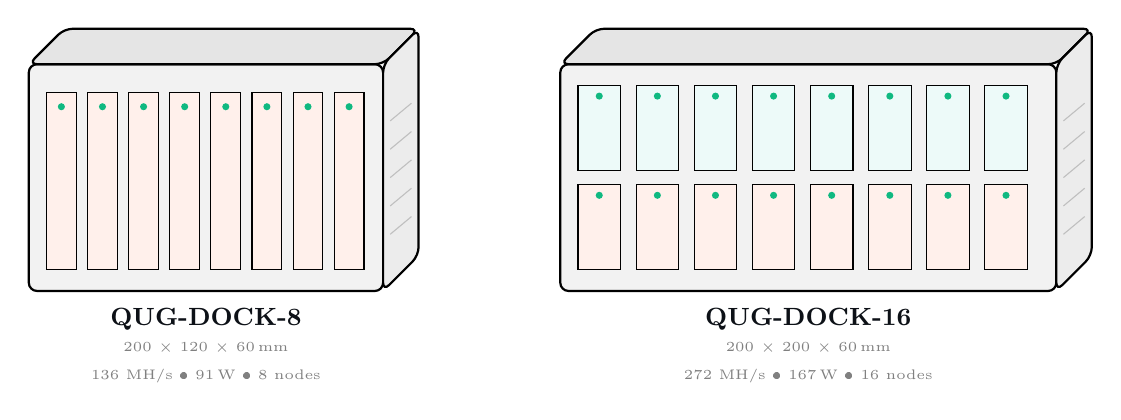
\begin{tikzpicture}[scale=0.9, every node/.style={font=\scriptsize}]
    % DOCK-8 (left)
    % 3D-ish box
    \draw[thick, fill=gray!10, rounded corners=3pt] (0,0) rectangle (5, 3.2);
    \draw[thick, fill=gray!20, rounded corners=3pt] (0,3.2) -- (0.5,3.7) -- (5.5,3.7) -- (5,3.2) -- cycle;
    \draw[thick, fill=gray!15, rounded corners=3pt] (5,0) -- (5.5,0.5) -- (5.5,3.7) -- (5,3.2) -- cycle;

    % Card slots visible from front
    \foreach \i in {0,...,7} {
        \pgfmathsetmacro{\sx}{0.25 + \i * 0.58}
        \draw[thin, fill=miningcolor!10] (\sx, 0.3) rectangle (\sx+0.42, 2.8);
        \fill[quggreen] (\sx+0.21, 2.6) circle (0.05);
    }

    % Labels
    \node[font=\small\bfseries, color=qnkdark] at (2.5, -0.4) {QUG-DOCK-8};
    \node[font=\tiny, color=gray] at (2.5, -0.8) {200 $\times$ 120 $\times$ 60\,mm};
    \node[font=\tiny, color=gray] at (2.5, -1.2) {136 MH/s \textbullet{} 91\,W \textbullet{} 8 nodes};

    % Ventilation holes on side
    \foreach \i in {0.8, 1.2, 1.6, 2.0, 2.4} {
        \draw[gray!50] (5.1, \i) -- (5.4, \i+0.25);
    }

    % DOCK-16 (right)
    \draw[thick, fill=gray!10, rounded corners=3pt] (7.5,0) rectangle (14.5, 3.2);
    \draw[thick, fill=gray!20, rounded corners=3pt] (7.5,3.2) -- (8.0,3.7) -- (15.0,3.7) -- (14.5,3.2) -- cycle;
    \draw[thick, fill=gray!15, rounded corners=3pt] (14.5,0) -- (15.0,0.5) -- (15.0,3.7) -- (14.5,3.2) -- cycle;

    % Two rows of 8 card slots
    \foreach \i in {0,...,7} {
        \pgfmathsetmacro{\sx}{7.75 + \i * 0.82}
        % Bottom row
        \draw[thin, fill=miningcolor!10] (\sx, 0.3) rectangle (\sx+0.6, 1.5);
        \fill[quggreen] (\sx+0.3, 1.35) circle (0.05);
        % Top row
        \draw[thin, fill=consensuscolor!10] (\sx, 1.7) rectangle (\sx+0.6, 2.9);
        \fill[quggreen] (\sx+0.3, 2.75) circle (0.05);
    }

    % Labels
    \node[font=\small\bfseries, color=qnkdark] at (11, -0.4) {QUG-DOCK-16};
    \node[font=\tiny, color=gray] at (11, -0.8) {200 $\times$ 200 $\times$ 60\,mm};
    \node[font=\tiny, color=gray] at (11, -1.2) {272 MH/s \textbullet{} 167\,W \textbullet{} 16 nodes};

    % Ventilation holes
    \foreach \i in {0.8, 1.2, 1.6, 2.0, 2.4} {
        \draw[gray!50] (14.6, \i) -- (14.9, \i+0.25);
    }
\end{tikzpicture}
\caption{Front view of QUG-DOCK-8 (8 slots, single row) and QUG-DOCK-16 (16 slots, dual row). Green LEDs indicate card presence and mining activity. Side vents provide airflow for the internal fans.}
\label{fig:dock_physical}
\end{figure}

\subsection{Dock Block Diagram}

\begin{figure}[H]
\centering
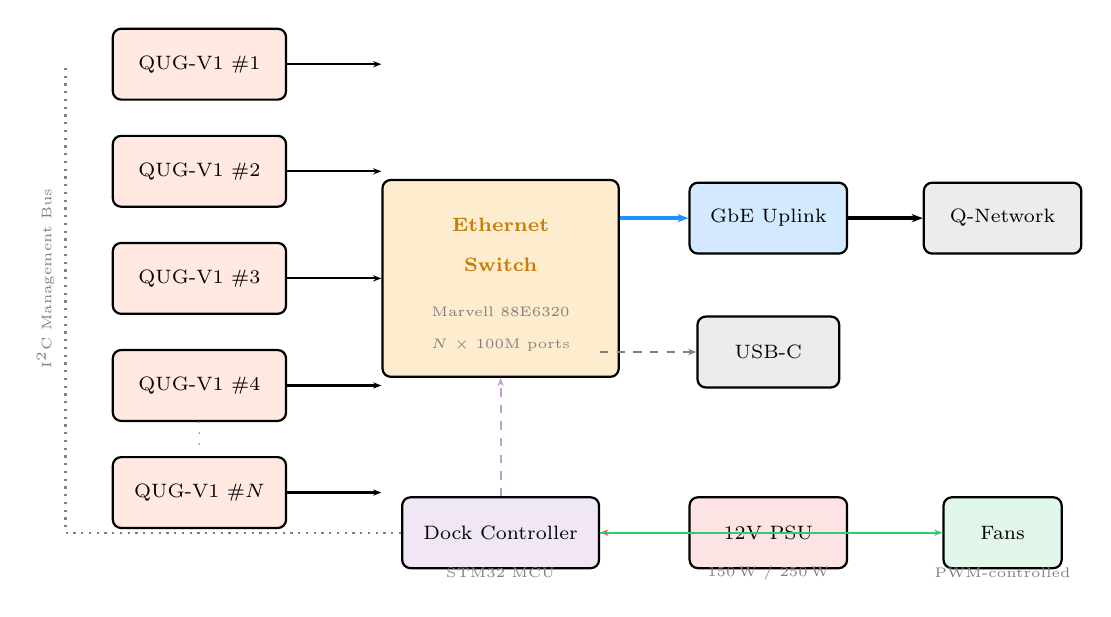
\begin{tikzpicture}[
    scale=0.85,
    block/.style={draw, thick, rounded corners=3pt, minimum height=0.9cm, font=\scriptsize, fill=#1},
    every node/.style={font=\scriptsize}
]
    % Cards
    \foreach \i in {0,...,3} {
        \pgfmathsetmacro{\yy}{4.8 - \i * 1.6}
        \node[block=miningcolor!15, minimum width=2.2cm] (card\i) at (0, \yy) {QUG-V1 \#\pgfmathparse{int(\i+1)}\pgfmathresult};
    }
    \node[font=\tiny, color=gray] at (0, -0.6) {$\vdots$};
    \node[block=miningcolor!15, minimum width=2.2cm] (cardN) at (0, -1.6) {QUG-V1 \#$N$};

    % Backplane switch
    \node[block=quggold!20, minimum width=3cm, minimum height=2.5cm] (switch) at (4.5, 1.6) {};
    \node[font=\scriptsize\bfseries, color=quggold!80!black] at (4.5, 2.4) {Ethernet};
    \node[font=\scriptsize\bfseries, color=quggold!80!black] at (4.5, 1.8) {Switch};
    \node[font=\tiny, color=gray] at (4.5, 1.1) {Marvell 88E6320};
    \node[font=\tiny, color=gray] at (4.5, 0.6) {$N$ $\times$ 100M ports};

    % Connections from cards to switch
    \foreach \i in {0,...,3} {
        \pgfmathsetmacro{\yy}{4.8 - \i * 1.6}
        \draw[thick, -{Stealth[length=3pt]}] (card\i.east) -- (switch.west |- card\i.east);
    }
    \draw[thick, -{Stealth[length=3pt]}] (cardN.east) -- (switch.west |- cardN.east);

    % Uplink
    \node[block=qnkblue!20, minimum width=2cm] (uplink) at (8.5, 2.5) {GbE Uplink};
    \draw[very thick, -{Stealth[length=4pt]}, color=qnkblue] (switch.east |- uplink) -- (uplink.west);

    % Internet
    \node[block=gray!15, minimum width=2cm] (inet) at (12, 2.5) {Q-Network};
    \draw[very thick, -{Stealth[length=4pt]}] (uplink.east) -- (inet.west);

    % Management MCU
    \node[block=pqcolor!15, minimum width=2.5cm] (mcu) at (4.5, -2.2) {Dock Controller};
    \node[font=\tiny, color=gray] at (4.5, -2.8) {STM32 MCU};
    \draw[thick, dashed, -{Stealth[length=3pt]}, color=pqcolor!60] (mcu.north) -- (switch.south);

    % I2C bus to cards
    \draw[thick, dotted, color=gray] (mcu.west) -| (-2, -2.2) -- (-2, 4.8);
    \node[font=\tiny, color=gray, rotate=90] at (-2.3, 1.6) {I$^2$C Management Bus};

    % PSU
    \node[block=qugred!15, minimum width=2cm] (psu) at (8.5, -2.2) {12V PSU};
    \draw[thick, color=qugred, -{Stealth[length=3pt]}] (psu.west) -- (mcu.east);
    \node[font=\tiny, color=gray] at (8.5, -2.8) {150\,W / 250\,W};

    % USB-C management
    \node[block=gray!15, minimum width=1.8cm] (usb) at (8.5, 0.5) {USB-C};
    \draw[thick, dashed, color=gray, -{Stealth[length=3pt]}] (mcu.east |- usb) -- (usb.west);

    % Fan control
    \node[block=iocolor!15, minimum width=1.5cm] (fans) at (12, -2.2) {Fans};
    \draw[thick, color=iocolor, -{Stealth[length=3pt]}] (mcu.east |- fans) -- (fans.west);
    \node[font=\tiny, color=gray] at (12, -2.8) {PWM-controlled};
\end{tikzpicture}
\caption{QUG-DOCK block diagram. Each QUG-V1 card connects to the managed Ethernet switch via the backplane edge connector. The dock controller monitors card health via I$^2$C and controls fan speed based on aggregate thermal load.}
\label{fig:dock_block}
\end{figure}

\subsection{Hot-Swap and Fault Tolerance}

The dock supports hot-swap card insertion and removal:

\begin{enumerate}
    \item \textbf{Insertion}: The dock controller detects card presence via I$^2$C, powers the slot, and the card boots autonomously (25-second boot time). The card's node joins the P2P network automatically via the Ethernet backplane.
    \item \textbf{Removal}: The card is power-gated by the dock controller. The network loses one peer; remaining cards continue unaffected. No data is lost---each card stores its blockchain state in its own LPDDR5X DRAM (volatile) and syncs from peers upon reinsertion.
    \item \textbf{Fault isolation}: If a card panics or overheats (junction temperature $> 105\,^\circ$C), the dock controller power-cycles that slot without affecting other cards. A persistent fault counter triggers a slot lockout after 3 consecutive failures.
\end{enumerate}

\begin{tcolorbox}[colback=green!5,colframe=quggreen,title=\textbf{Decentralization Benefit}]
A QUG-DOCK-16 running in \textbf{Independent mode} contributes 16 full nodes to the Q-NarwhalKnight network---each with its own peer identity, its own copy of the blockchain, and its own vote in consensus. This is equivalent to 16 separate Raspberry Pi nodes in a single quiet, compact enclosure. Unlike GPU mining rigs that centralize hashrate without contributing nodes, every QUG-V1 card strengthens the network's decentralization.
\end{tcolorbox}

% ═══════════════════════════════════════════════════════════════════
\section{Comparative Analysis}
\label{sec:comparison}
% ═══════════════════════════════════════════════════════════════════

\subsection{Platform Comparison}

\begin{table}[H]
\centering
\caption{QUG-V1 vs. Alternative Mining Platforms}
\label{tab:comparison}
\begin{tabular}{@{}lrrrrrrr@{}}
\toprule
\textbf{Metric} & \textbf{QUG-V1} & \textbf{DOCK-8} & \textbf{DOCK-16} & \textbf{RPi 5} & \textbf{RTX 4090} & \textbf{BTC ASIC} \\
 & \textbf{(1 card)} & \textbf{(8 cards)} & \textbf{(16 cards)} & & & \textbf{(S21 XP)} \\
\midrule
QUG Hashrate & 17 MH/s & 136 MH/s & 272 MH/s & 200 kH/s & 5 MH/s$^\dagger$ & N/A$^\ddagger$ \\
Power & 9.5 W & 91 W & 167 W & 12 W & 450 W & 3,583 W \\
Efficiency & 1.79 MH/J & 1.49 MH/J & 1.63 MH/J & 17 kH/J & 11 kH/J & N/A \\
Price & \$149--199 & \$1,300 & \$2,550 & \$80 & \$1,999 & \$5,000+ \\
Form factor & Credit card & Shoebox & Shoebox & SBC & PCIe & Rack unit \\
Full nodes & 1 & 8 & 16 & 1 & 0 & 0 \\
PQ-ready? & Yes (HW) & Yes (HW) & Yes (HW) & Partial & No & No \\
Noise level & Silent & $<$30 dB & $<$35 dB & Silent & 50+ dB & 75+ dB \\
\bottomrule
\end{tabular}

\vspace{0.3cm}
{\footnotesize $^\dagger$GPU parallelism limited by VDF sequential chain. $^\ddagger$Bitcoin ASICs compute SHA-256, incompatible with QUG's BLAKE3+VDF.}
\end{table}

\subsection{Why GPUs Cannot Compete}

The VDF chain in QUG mining creates a fundamental asymmetry:

\begin{theorem}[GPU Parallelism Limitation]
Let a GPU have $P$ shader cores. For QUG mining, the effective parallelism is limited to independent nonce evaluations (not intra-nonce parallelism):
\begin{equation}
    \text{GPU throughput} = P \times \frac{f_{\text{GPU}}}{C_{\text{nonce}}^{\text{GPU}}}
\end{equation}
where $C_{\text{nonce}}^{\text{GPU}} \gg C_{\text{nonce}}^{\text{QUG-V1}}$ because:
\begin{enumerate}
    \item GPU BLAKE3 is software-only ($\sim$50 cycles/hash vs.\ 9 on QUG-V1).
    \item GPU shader cores run at $\sim$2\,GHz but share memory bandwidth.
    \item VDF prevents SIMD vectorization within a single nonce.
\end{enumerate}
An NVIDIA RTX 4090 (16,384 cores, 2.52\,GHz) achieves $\sim$5\,MH/s on QUG at 450\,W---yielding 11\,kH/s/W, which is $163\times$ less efficient than the QUG-V1.
\end{theorem}

\subsection{Radar Comparison}

\begin{figure}[H]
\centering
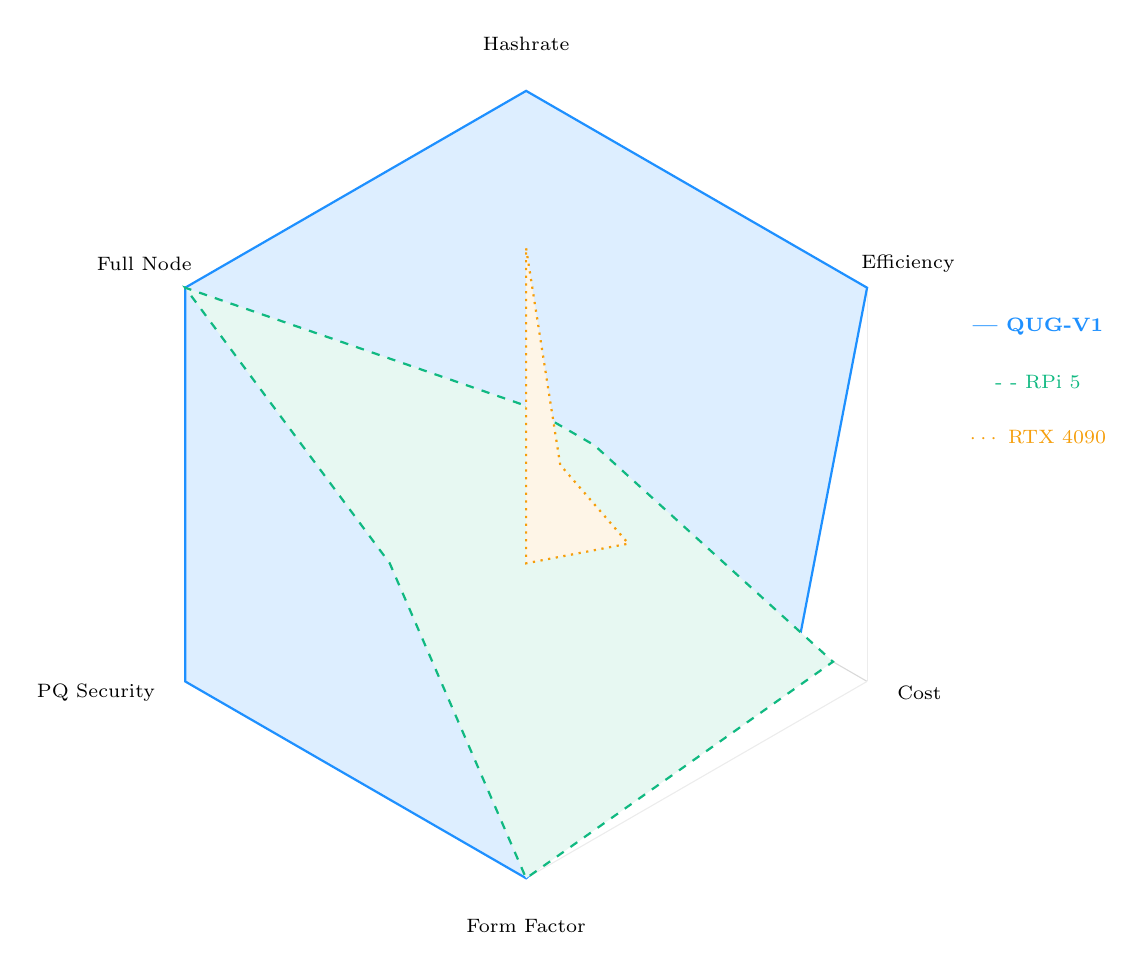
\begin{tikzpicture}[scale=1.0]
    % Axes
    \def\axes{6}
    \def\maxval{5}
    \foreach \i in {1,...,\axes} {
        \pgfmathsetmacro{\angle}{90 - (\i - 1) * 360 / \axes}
        \draw[gray!30] (0,0) -- (\angle:\maxval);
        % Concentric pentagons
        \foreach \r in {1,...,5} {
            \pgfmathsetmacro{\nexti}{\i + 1}
            \ifnum\i<\axes
                \pgfmathsetmacro{\nextangle}{90 - \i * 360 / \axes}
                \draw[gray!15] (\angle:\r) -- (\nextangle:\r);
            \else
                \draw[gray!15] (\angle:\r) -- (90:\r);
            \fi
        }
    }

    % Labels
    \node[font=\scriptsize] at (90:5.6) {Hashrate};
    \node[font=\scriptsize] at (30:5.6) {Efficiency};
    \node[font=\scriptsize, anchor=west] at (-30:5.3) {Cost};
    \node[font=\scriptsize] at (-90:5.6) {Form Factor};
    \node[font=\scriptsize, anchor=east] at (210:5.3) {PQ Security};
    \node[font=\scriptsize] at (150:5.6) {Full Node};

    % QUG-V1 (blue)
    \draw[thick, qnkblue, fill=qnkblue!15]
        (90:5) -- (30:5) -- (-30:4) -- (-90:5) -- (210:5) -- (150:5) -- cycle;

    % RPi 5 (green)
    \draw[thick, quggreen, fill=quggreen!10, dashed]
        (90:1) -- (30:1) -- (-30:4.5) -- (-90:5) -- (210:2) -- (150:5) -- cycle;

    % RTX 4090 (gold)
    \draw[thick, quggold, fill=quggold!10, dotted]
        (90:3) -- (30:0.5) -- (-30:1.5) -- (-90:1) -- (210:0) -- (150:0) -- cycle;

    % Legend
    \node[font=\scriptsize, color=qnkblue] at (6.5, 2) {\textbf{--- QUG-V1}};
    \node[font=\scriptsize, color=quggreen] at (6.5, 1.3) {- - RPi 5};
    \node[font=\scriptsize, color=quggold] at (6.5, 0.6) {$\cdots$ RTX 4090};
\end{tikzpicture}
\caption{Radar comparison across six axes (5 = best). The QUG-V1 dominates in hashrate, efficiency, PQ security, and full node capability while matching the RPi 5 in form factor and cost.}
\label{fig:radar}
\end{figure}

% ═══════════════════════════════════════════════════════════════════
\section{Conclusion and Roadmap}
\label{sec:conclusion}
% ═══════════════════════════════════════════════════════════════════

\subsection{Summary}

The QUG-V1 demonstrates that purpose-built hardware can deliver transformative efficiency gains for the Q-NarwhalKnight blockchain:

\begin{itemize}
    \item \textbf{17\,MH/s} mining throughput---$85\times$ faster than a Raspberry Pi 5
    \item \textbf{9.5\,W} power consumption---passively cooled, silent operation
    \item \textbf{1.79\,MH/s/W}---$107\times$ more efficient than general-purpose hardware
    \item \textbf{Full node} capability---no separate server required
    \item \textbf{Post-quantum ready}---hardware Dilithium5 and Kyber1024 acceleration
    \item \textbf{\$149--199} retail price---accessible to individual users
    \item \textbf{\$8.33/year} operating cost---profitable even at minimal network share
    \item \textbf{Rust-only stack}---from RTL to application, a single verified toolchain
    \item \textbf{QUG-DOCK} scalability---8 or 16 cards in a compact enclosure for 136--272\,MH/s
\end{itemize}

By packaging a complete mining node into a credit-card form factor, the QUG-V1 lowers the barrier to network participation from ``deploy a server'' to ``plug in a USB-C cable.'' For operators who want more hashrate, the QUG-DOCK scales linearly to 272\,MH/s while contributing up to 16 independent full nodes to the network. This democratization of mining is essential for the long-term decentralization and security of the Q-NarwhalKnight network.

\subsection{Development Roadmap}

\begin{table}[H]
\centering
\caption{QUG-V1 Development Roadmap}
\begin{tabular}{@{}lllp{7cm}@{}}
\toprule
\textbf{Phase} & \textbf{Target} & \textbf{Milestone} & \textbf{Description} \\
\midrule
1 & 2026 Q3 & FPGA Prototype & Xcrypto BLAKE3 extension validated on Xilinx Artix-7. Full mining pipeline at 100\,MHz ($\sim$1\,MH/s). Bare-metal firmware boots and mines. \\
\addlinespace
2 & 2027 Q1 & TSMC 7nm Tape-out & First silicon with all 16 cores. Conservative 7\,nm process for yield optimization. Target: 10\,MH/s at 12\,W. \\
\addlinespace
3 & 2027 Q3 & TSMC 5nm + DOCK & Volume production on N5. Full 17\,MH/s at 9.5\,W. Credit-card form factor finalized. QUG-DOCK-8 and DOCK-16 enclosures ship alongside cards. First \$149 retail units. \\
\addlinespace
4 & 2028 & QUG-V2 + DOCK-V2 & Second-gen card: QRNG for Tor circuit seeding, SQIsign isogeny accelerator, integrated Wi-Fi. 50\,MH/s at 8\,W. DOCK-V2: 10GbE uplink, NVMe slot for persistent blockchain storage, PoE+ per-slot power. \\
\bottomrule
\end{tabular}
\end{table}

\subsection{Open Source Commitment}

The QUG-V1 design will be released under permissive open-source licenses:

\begin{itemize}
    \item \textbf{RTL source} (\texttt{rust-hdl}): Apache 2.0 / MIT dual-license
    \item \textbf{Firmware}: Apache 2.0 / MIT (same as Q-NarwhalKnight workspace)
    \item \textbf{ISA extensions} (Xcrypto, Xlattice): RISC-V Foundation contribution
    \item \textbf{PCB design files}: Creative Commons BY-SA 4.0
\end{itemize}

This ensures that any community member can audit the hardware, build custom firmware, or manufacture compatible devices---reinforcing the decentralization ethos of the Q-NarwhalKnight network.

\vspace{1cm}
\hrule
\vspace{0.5cm}
\begin{center}
\textit{``The best way to predict the future is to invent it.''}\\
--- Alan Kay
\end{center}

% ═══════════════════════════════════════════════════════════════════
\appendix
\section{Xcrypto Instruction Encoding}
\label{app:xcrypto}
% ═══════════════════════════════════════════════════════════════════

The Xcrypto extension uses the RISC-V custom-0 opcode space. Instruction encodings:

\begin{table}[H]
\centering
\caption{Xcrypto Instruction Encoding (R-type format)}
\small
\begin{tabular}{@{}lcccccc@{}}
\toprule
\textbf{Instruction} & \textbf{funct7} & \textbf{rs2} & \textbf{rs1} & \textbf{funct3} & \textbf{rd} & \textbf{opcode} \\
\midrule
\texttt{blake3.init} & 0000000 & 00000 & 00000 & 000 & 00000 & 0001011 \\
\texttt{blake3.round} & 0000001 & 00000 & 00000 & 000 & 00000 & 0001011 \\
\texttt{blake3.chain} & 0000010 & 00000 & 00000 & 000 & 00000 & 0001011 \\
\texttt{blake3.finalize} & 0000011 & rs1 & 00000 & 000 & rd & 0001011 \\
\bottomrule
\end{tabular}
\end{table}

\section{Xlattice Instruction Encoding}
\label{app:xlattice}

\begin{table}[H]
\centering
\caption{Xlattice Instruction Encoding (R-type format)}
\small
\begin{tabular}{@{}lcccccc@{}}
\toprule
\textbf{Instruction} & \textbf{funct7} & \textbf{rs2} & \textbf{rs1} & \textbf{funct3} & \textbf{rd} & \textbf{opcode} \\
\midrule
\texttt{ntt.fwd} & 0000000 & rs2 & rs1 & 000 & rd & 0101011 \\
\texttt{ntt.inv} & 0000001 & rs2 & rs1 & 000 & rd & 0101011 \\
\texttt{poly.add} & 0000010 & rs2 & rs1 & 000 & rd & 0101011 \\
\texttt{poly.mul} & 0000011 & rs2 & rs1 & 000 & rd & 0101011 \\
\texttt{poly.reduce} & 0000100 & 00000 & rs1 & 000 & rd & 0101011 \\
\bottomrule
\end{tabular}
\end{table}

\section{Complete Power Model}
\label{app:power}

The power model uses standard CMOS dynamic and static power equations:

\begin{align}
    P_{\text{dynamic}} &= \alpha \cdot C_{\text{eff}} \cdot V_{dd}^2 \cdot f \\
    P_{\text{static}} &= V_{dd} \cdot I_{\text{leak}} \cdot N_{\text{transistors}}
\end{align}

For TSMC N5 at $V_{dd} = 0.75$\,V:

\begin{table}[H]
\centering
\caption{Detailed Power Model Parameters}
\small
\begin{tabular}{@{}lrrrr@{}}
\toprule
\textbf{Block} & $\alpha$ & $C_{\text{eff}}$ (nF) & $f$ (GHz) & $P$ (mW) \\
\midrule
RV64GC core & 0.15 & 2.0 & 1.5 & 254 \\
Xcrypto BLAKE3 unit & 0.40 & 1.5 & 1.5 & 405 \\
RVV 256-bit SIMD & 0.20 & 3.0 & 1.5 & 506 \\
Xlattice NTT engine & 0.25 & 2.5 & 1.2 & 422 \\
L1 cache (64\,KB) & 0.10 & 0.5 & 1.5 & 42 \\
L2 cache (1\,MB) & 0.05 & 2.0 & 1.5 & 84 \\
L3 cache (16\,MB) & 0.03 & 10.0 & 1.5 & 253 \\
NoC router & 0.08 & 0.3 & 1.5 & 20 \\
\bottomrule
\end{tabular}
\end{table}

\section{BLAKE3 Algorithm Reference}
\label{app:blake3}

For completeness, we summarize the BLAKE3 compression function as implemented in the Xcrypto hardware:

\begin{definition}[BLAKE3 Quarter Round]
Operating on state words $a, b, c, d$ (each 32 bits):
\begin{align}
    a &\leftarrow a + b + m_x \\
    d &\leftarrow (d \oplus a) \ggg 16 \\
    c &\leftarrow c + d \\
    b &\leftarrow (b \oplus c) \ggg 12 \\
    a &\leftarrow a + b + m_y \\
    d &\leftarrow (d \oplus a) \ggg 8 \\
    c &\leftarrow c + d \\
    b &\leftarrow (b \oplus c) \ggg 7
\end{align}
where $m_x, m_y$ are message schedule words and $\ggg$ denotes right rotation.
\end{definition}

Each BLAKE3 round applies 8 quarter-rounds to the 16-word state (4 column rounds + 4 diagonal rounds). The Xcrypto unit computes all 8 quarter-rounds in parallel using 8 independent 32-bit ALU lanes, completing one round per clock cycle.

\end{document}
